\documentclass[11pt,a4paper]{article}

\usepackage[utf8]{inputenc}
\usepackage[T1]{fontenc}
\usepackage[english]{babel}
\usepackage[margin=2.5cm]{geometry}
\usepackage{amsmath, amssymb}
\usepackage{graphicx}
\usepackage{booktabs}
\usepackage{array}
\usepackage{enumitem}
\usepackage{xcolor}
\usepackage{tikz}
\usetikzlibrary{positioning, arrows.meta, shapes.geometric, fit}
\usepackage[ruled,vlined,linesnumbered]{algorithm2e}
\usepackage{hyperref}
\hypersetup{colorlinks=true, linkcolor=black, citecolor=black, urlcolor=blue}
\usepackage{caption}
\captionsetup{font=small, labelfont=bf}
\usepackage[normalem]{ulem}

\newcolumntype{L}[1]{>{\raggedright\arraybackslash}p{#1}}
\newcommand{\code}[1]{\texttt{#1}}

% Give TeX a little extra slack so long unbreakable code/file names and
% math-joined words can be pushed to the next line instead of overflowing.
\setlength{\emergencystretch}{3em}

% Experimental numbers generated by plot_results.py — never hand-typed.
\newcommand{\cmpHorizon}{10}
\newcommand{\cmpFinalYear}{2035}
\newcommand{\cmpModel}{neural}
\newcommand{\cmpSeeds}{3}
\newcommand{\baseGdp}{274.6}
\newcommand{\baseGini}{0.439}
\newcommand{\baseWorst}{230.1}
\newcommand{\cmpUtilGdp}{301.6}
\newcommand{\cmpUtilGdpStd}{18.3}
\newcommand{\cmpUtilGini}{0.436}
\newcommand{\cmpUtilGiniStd}{0.001}
\newcommand{\cmpUtilWorst}{243.1}
\newcommand{\cmpUtilWorstStd}{25.5}
\newcommand{\cmpUtilGdpDelta}{+9.8}
\newcommand{\cmpUtilWorstDelta}{+5.6}
\newcommand{\cmpUtilTrainImpr}{+24.0}
\newcommand{\cmpRawlsGdp}{254.7}
\newcommand{\cmpRawlsGdpStd}{24.5}
\newcommand{\cmpRawlsGini}{0.380}
\newcommand{\cmpRawlsGiniStd}{0.009}
\newcommand{\cmpRawlsWorst}{268.4}
\newcommand{\cmpRawlsWorstStd}{4.3}
\newcommand{\cmpRawlsGdpDelta}{-7.3}
\newcommand{\cmpRawlsWorstDelta}{+16.6}
\newcommand{\cmpRawlsTrainImpr}{+26.6}
\newcommand{\cmpCvarGdp}{257.6}
\newcommand{\cmpCvarGdpStd}{7.0}
\newcommand{\cmpCvarGini}{0.368}
\newcommand{\cmpCvarGiniStd}{0.013}
\newcommand{\cmpCvarWorst}{268.9}
\newcommand{\cmpCvarWorstStd}{7.1}
\newcommand{\cmpCvarGdpDelta}{-6.2}
\newcommand{\cmpCvarWorstDelta}{+16.9}
\newcommand{\cmpCvarTrainImpr}{+26.7}
\newcommand{\cmpEgalGdp}{302.3}
\newcommand{\cmpEgalGdpStd}{2.7}
\newcommand{\cmpEgalGini}{0.417}
\newcommand{\cmpEgalGiniStd}{0.001}
\newcommand{\cmpEgalWorst}{268.6}
\newcommand{\cmpEgalWorstStd}{7.7}
\newcommand{\cmpEgalGdpDelta}{+10.1}
\newcommand{\cmpEgalWorstDelta}{+16.7}
\newcommand{\cmpEgalTrainImpr}{+25.2}
\newcommand{\cmpWellGdp}{294.1}
\newcommand{\cmpWellGdpStd}{11.3}
\newcommand{\cmpWellGini}{0.421}
\newcommand{\cmpWellGiniStd}{0.011}
\newcommand{\cmpWellWorst}{255.5}
\newcommand{\cmpWellWorstStd}{12.6}
\newcommand{\cmpWellGdpDelta}{+7.1}
\newcommand{\cmpWellWorstDelta}{+11.0}
\newcommand{\cmpWellTrainImpr}{+90.5}
\newcommand{\parPoints}{14}
\newcommand{\parEvals}{84}
\newcommand{\parGens}{6}
\newcommand{\parPop}{12}
\newcommand{\parGdpSpanLo}{233.7}
\newcommand{\parGdpSpanHi}{321.0}
\newcommand{\parGiniLo}{0.439}
\newcommand{\parGiniHi}{0.439}
\newcommand{\parGiniSpanMicro}{7}
\newcommand{\parWorstLo}{195.9}
\newcommand{\parWorstHi}{269.0}
\newcommand{\parCorr}{1.000}
\newcommand{\parcPoints}{3}
\newcommand{\parcClusters}{4}
\newcommand{\parcGdpSpanLo}{302.7}
\newcommand{\parcGdpSpanHi}{321.2}
\newcommand{\parcGiniLo}{0.411}
\newcommand{\parcGiniHi}{0.418}
\newcommand{\parcWorstLo}{269.5}
\newcommand{\parcWorstHi}{281.4}
\newcommand{\provTotal}{24}
\newcommand{\provMeasured}{11}
\newcommand{\provDisaggNational}{7}
\newcommand{\provDisaggRegional}{6}
\newcommand{\provDisaggTotal}{13}
\newcommand{\provGdp}{disaggregated regional}


\title{\textbf{SERA: An Ethically-Governed Digital Twin of the
Italian Provinces:\\ Comparing Distributive-Justice Objectives in
AI Policy Optimization}\\[1ex]
\large Ethics in Artificial Intelligence}
\author{Leonardo Tassinari\\
University of Bologna\\
Master in Artificial Intelligence\\
\texttt{leonardo.tassinari6@studio.unibo.it}}
\date{June 2026}

\begin{document}

\maketitle

\begin{abstract}
This project studies the ethical governance of an AI system that advises on the
allocation of public resources. SERA (Socio-Economic Resource Allocator) is a \emph{digital twin} of the 110 Italian
provinces: it ingests $\sim$88 historical socioeconomic indicators (2001--2025)
from the Italian National Institute of Statistics (ISTAT), trains one machine
learning model per indicator, and simulates the provinces forward year by year
under user-chosen policy levers (tax rates, spending allocations, regulatory
settings) subject to a national budget constraint. On top of the twin, an AI
policy optimizer searches for multi-year lever settings, but \emph{what} it
maximizes is an explicit, user-facing ethical choice among four pluggable
objectives drawn from theories of distributive justice: Utilitarianism (total
GDP), Rawlsian justice (maximin), Egalitarianism (Sen welfare), and a
multi-indicator wellbeing composite. The optimizer itself is also a choice,
spanning a deliberate \emph{explainability spectrum} from white-box rule lists
to a black-box neural policy audited post hoc, so that the price of transparency
is measured rather than assumed. A multi-objective Pareto-frontier search
(NSGA-II) reframes the efficiency--equity trade-off as a continuum instead of a
dropdown. The system is wrapped in responsible-AI scaffolding, ethics
statement, model card, datasheet, sensitivity bands, and a human-in-the-loop
candidate/adopt workflow, and positioned explicitly with respect to the EU AI
Act. The report includes an experimental comparison in which the same neural
policy model is trained once per ethical framework from the same 2025 starting
state and rolled out to \cmpFinalYear{}, replicated across several seeds: the
frameworks drive the same optimizer to measurably different futures: the
distribution-blind utilitarian run grows the average most but leaves the
worst-off province the lowest of the interventions, while maximin (and a smoothed
Conditional-Value-at-Risk variant added to test its sparse signal) reliably
raises the floor and reproduces the leveling-down objection by cutting the
richest tail, and Sen welfare buys the highest floor among the growth-positive
options. A methodological result falls out of the replication: a single seed
had shown maximin's floor falling \emph{below} the utilitarian one, a tidy
story that dissolved under replication as search luck. The NSGA-II search then
reveals that \emph{uniform} national policy cannot trade efficiency against
inequality at all, while a clustered search that can target regions makes the
trade-off reappear: distributional outcomes are determined by per-province
\emph{targeting}. Read in the dimension that motivated the choice of Italy
(the North--South divide), the frameworks separate cleanly: the utilitarian
tide leaves the gap untouched, maximin closes it by leveling the North down, and
only Sen welfare narrows it while both regions grow. The project's central claim
is that an optimizer always
embodies an ethical framework; SERA's contribution is to make that framework
visible, swappable, and inspectable.
\end{abstract}

\tableofcontents
\newpage

\section{Introduction}

Artificial Intelligence systems are increasingly consulted in decisions that
allocate resources among people: budget planning, service provisioning, urban
management, welfare administration. Whenever such a system recommends \emph{who
gets what}, it is not merely performing a technical optimization; it is
enacting a theory of distributive justice, whether its designers acknowledge it
or not. An optimizer that maximizes total output is a utilitarian; one that
protects the worst-off is Rawlsian; one that penalizes inequality is
egalitarian. The objective function is a value judgment wearing the costume of
mathematics, and the costume is effective: a number that emerges from a
pipeline of models reads as neutral in a way that the same judgment, stated in
words, never would.

This project confronts that observation directly. SERA (the name plays on the
Italian \emph{sera} and is the acronym for ``Socio-Economic Resource Allocator'') is a digital twin of the Italian provinces. Italy is an ideal
testbed for distributive questions: the North--South divide is one of the most
persistent regional inequalities in Europe, and any national policy implicitly
chooses between aggregate growth and territorial cohesion. SERA simulates the
socioeconomic trajectories of the 110 provinces under user-controlled policy
levers, and lets an AI optimizer propose lever settings over a multi-year
horizon. Crucially, the system separates three questions that are usually
conflated:

\begin{enumerate}
    \item \textbf{What does the world do?} The twin: per-indicator ML models
    plus a causal graph that is hand-written but \emph{panel-reviewed} (its edge
    directions checked against, and corrected by, the historical data;
    Section~\ref{sec:datareview}), with honestly documented uncertainty.
    \item \textbf{How do we search?} The policy model: seven optimizers
    spanning an explainability spectrum from printable IF/THEN rules to a neural
    network.
    \item \textbf{What counts as better?} The ethical objective: four
    pluggable formalizations of distributive justice, plus a Pareto frontier
    that searches all of them at once.
\end{enumerate}

Because any policy model can be paired with any objective, the distributional
consequences of each ethical framework become directly comparable on the same
model of the same country: what Utilitarianism does to the map, what Rawlsian
maximin is willing to sacrifice, and how Sen welfare negotiates between them
become empirical questions rather than positions. This report carries out
that comparison experimentally (Section~\ref{sec:results}): the same neural
policy is trained once per framework from the same starting state, and the
resulting futures are compared on efficiency, inequality, and the floor,
with results that match the textbook in some places and instructively depart
from it in others.

The challenge this prototype abstracts is practical and current. Key real-world
analogues include:

\begin{itemize}
    \item \textbf{Regional development funds}: allocating EU cohesion or
    national recovery funds (e.g., Italy's PNRR) across territories, where the
    tension between efficiency and territorial equity is the explicit subject of
    political debate.
    \item \textbf{Public-service capacity planning}: distributing healthcare or
    education investment across regions with different returns and different
    needs.
    \item \textbf{Algorithmic benefit administration}: any scoring system that
    prioritizes applicants or regions for limited funds embodies the same
    choice between total measured benefit and protection of the worst placed.
\end{itemize}

SERA is decision \emph{support}, never decision \emph{making}: the optimizer
returns graded candidates with stated trade-offs, and a human must explicitly
adopt one, including, as a first-class option, doing nothing. The report
proceeds as follows. Section~\ref{sec:background} places the project in the
machine-ethics landscape. Sections~\ref{sec:tech}--\ref{sec:system} present the
technologies and the system design. Section~\ref{sec:theory} analyzes the
implemented ethical frameworks philosophically and algorithmically, including
the frameworks considered but not implemented.
Section~\ref{sec:policymodels} details the policy-model spectrum and its
mathematics; Section~\ref{sec:explain} discusses explainability as an ethical
design axis; Section~\ref{sec:oversight} covers human oversight, uncertainty,
documentation, and the EU AI Act. Section~\ref{sec:results} presents the
experimental comparison of the four frameworks and the Pareto frontier;
Section~\ref{sec:discussion} discusses the findings and their limits;
Section~\ref{sec:conclusions} concludes. Reproducibility instructions are in
Section~\ref{sec:repro}, and the appendix lists the core algorithms.

\section{Background: Machine Ethics and Value-Laden Optimization}
\label{sec:background}

Moor's influential taxonomy of machine ethics~\cite{moor2006} distinguishes
\emph{ethical-impact agents} (any machine whose use has ethical consequences),
\emph{implicit ethical agents} (machines whose safe behavior is built into
their design), and \emph{explicit ethical agents} (machines that represent
ethical categories and reason over them). Most deployed optimization systems
are ethical-impact agents pretending to be neither: their objective function
encodes a moral stance, usually an unexamined sum-maximization, without
representing it as such. SERA's design goal is to move one deliberate step up
Moor's ladder: the ethical framework is reified as a first-class software
object (an \code{Objective} class with an identifier, a label, and an honest
natural-language description of what it ignores), selected by a human before
any optimization runs. The machine does not \emph{reason} about ethics (the
choice of framework remains human), but the framework is explicit,
inspectable, and swappable, rather than implicit in a hard-coded loss.

Three adjacent literatures inform the design. First, the \emph{fairness in
machine learning} literature has established that fairness admits multiple,
mutually incompatible formalizations and that the choice among them is
normative, not technical; SERA transposes that lesson from classification
(individual versus group fairness) to resource allocation (utilitarian versus
maximin versus inequality-discounted welfare). Second, the \emph{AI governance}
literature converges on a small set of principles: transparency, justice,
non-maleficence, responsibility, privacy~\cite{jobin2019}, which SERA
operationalizes as concrete artifacts: explainability badges, an ethics
statement, a model card~\cite{mitchell2019}, a datasheet~\cite{gebru2021}, and
an explicit EU AI Act mapping~\cite{aiact2024}. Third, the \emph{beyond-GDP}
movement in welfare economics~\cite{stiglitz2009} supplies the critique that
motivates the fourth objective: even a perfectly fair distribution of the wrong
quantity is the wrong target.

A note on what SERA is not. It is not an attempt to build an artificial moral
agent, nor to learn ethics from data: the frameworks are classical theories of
distributive justice, hand-formalized, and the system's contribution is
comparative infrastructure, the ability to hold everything else fixed while
swapping the moral criterion, which philosophy can rarely do and policy
experiments can never do.

\section{Employed Technologies}
\label{sec:tech}

\subsection{Python and the scientific stack}

The data pipeline and the twin engine are implemented in Python~3.11. The
indicator models use \code{scikit-learn} (ridge regression by default, random
forests as an alternative); the simulator, the gradient-free policy optimizers,
and the NSGA-II search are written in \code{NumPy}/\code{pandas} with no
deep-learning framework, the ``neural'' policy is a small pure-NumPy
multilayer perceptron, trained by evolution strategies rather than
backpropagation, since the twin it must optimize through is a
non-differentiable composite of sklearn models and hand-written rules. Trained
models are persisted with \code{joblib}.

\subsection{The ISTAT SDMX API}

All historical data comes from the official SDMX API of ISTAT, the Italian
National Institute of Statistics. The client (\code{sera.istat\_client}) is
rate-limited, ISTAT enforces a hard limit of 5 requests/minute per IP, and
exceeding it can lead to multi-day IP bans, so the client keeps a 25-second
minimum delay between requests, counting failed requests too, and caches
every response keyed by dataflow, dimensional key, and year range, so that a
given data snapshot is preserved even though ISTAT revises history. A known
quirk of the API (the \code{endPeriod} parameter returns year$+1$) is
compensated for centrally. Each downloaded series carries a
\code{.mapping.json} sidecar recording exactly which ISTAT dataflow and
dimensions produced it, keeping every number traceable to its official source,
a provenance requirement that the datasheet (Section~\ref{sec:docs})
elevates from engineering hygiene to data governance.

\subsection{Electron + React control-room UI}

The user interface is an Electron desktop application with a React front end: a
clickable province map (GeoJSON choropleth), per-province policy allocators, a
national budget meter, the optimizer panel, an ethics equity dashboard, and the
Pareto-frontier view. All JavaScript libraries are vendored; the app makes no
network requests at runtime. The Electron main process talks to Python through a
bridge script (\code{ui/backend\_bridge.py}), one process per command
(\code{bootstrap}, \code{province-trends}, \code{simulate-next-year},
\code{optimize-policy}, \code{compare-objectives}, \code{pareto-front}),
streaming structured progress messages over \code{stderr}.

\subsection{Pytest}

The mechanics of the system, indicator bounds, the budget constraint,
objective arithmetic, Pareto dominance, determinism of the policy optimizers,
province-code normalization, are covered by a \code{pytest} suite. The tests
deliberately cover \emph{mechanics, not predictive accuracy}: asserting that the
twin forecasts Italy correctly would be a claim the project explicitly refuses
to make (Section~\ref{sec:uncertainty}).
The tests are run automatically on every commit by GitHub Actions and gitlab CI, and the system refuses to run if any test fails.

\section{The System}
\label{sec:system}

\subsection{Project structure}

\begin{itemize}
    \item \code{src/sera/}: the Python package.
    \begin{itemize}
        \item \code{config.py}: paths, ISTAT constants, the
        indicator$\to$category map.
        \item \code{istat\_client.py}, \code{downloader.py},
        \code{downloaders/<category>/<indicator>.py}: the rate-limited,
        cached data pipeline; one module per indicator.
        \item \code{twin/}: the digital twin:
        \begin{itemize}
            \item \code{data\_loader.py}: panel assembly, disaggregation,
            interpolation;
            \item \code{model\_trainer.py}: one regressor per indicator;
            \item \code{causal\_graph.py}: 20 policy levers, their documented
            lever$\to$indicator links, inter-indicator dependencies, bounds and
            effect directions;
            \item \code{simulator.py}: the year-step engine;
            \item \code{budget.py}: the national budget constraint (pool,
            tax funding, reserve carry-over), a pure package module so the
            headless experiments need not import the UI layer;
            \item \code{policy.py}: the rollout environment, the budget
            constraint seam, and the seven policy models;
            \item \code{objectives.py}: the seven ethical objectives;
            \item \code{explain.py}: post-hoc audits for black-box policies;
            \item \code{pareto.py}: the NSGA-II efficiency--equity frontier
            (uniform or per-cluster);
            \item \code{panel\_estimation.py}: fixed-effects panel estimation
            that re-derives the twin's structure from the data, scores it against
            the hand-written graph, and produces the reviewed edge signs the
            simulator consumes (Section~\ref{sec:datareview});
            \item \code{cli.py}: training and batch simulation.
        \end{itemize}
    \end{itemize}
    \item \code{ui/}: the Electron app (\code{main.js}, \code{preload.js},
    \code{renderer.js}, \code{backend\_bridge.py}).
    \item \code{data/}: downloaded indicator CSVs (110 provinces, 2-letter
    sigle).
    \item \code{ETHICS.md}, \code{docs/MODEL\_CARD.md}, \code{docs/DATASHEET.md},
the responsible-AI documentation (Section~\ref{sec:docs}).
    \item \code{tests/}: the pytest suite.
    \item \code{report/}: this report, with the experiment scripts
    (\code{run\_\allowbreak experiments.py}, \code{plot\_\allowbreak results.py}) that generated
    Section~\ref{sec:results}.
\end{itemize}

\begin{figure}[ht]
\centering
\resizebox{\textwidth}{!}{%
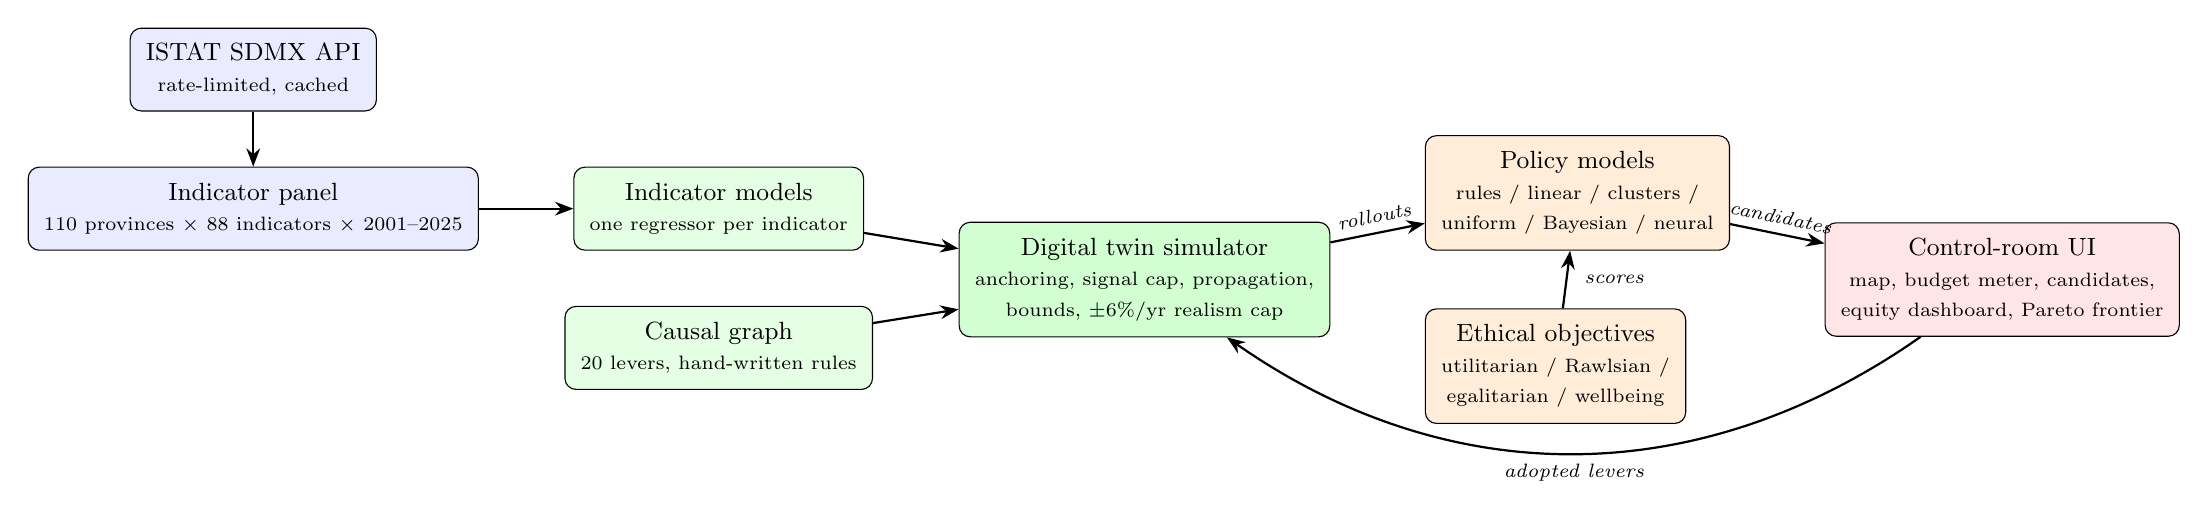
\begin{tikzpicture}[
    node distance=7mm and 12mm,
    box/.style={rectangle, rounded corners, draw, align=center,
                minimum height=9mm, inner sep=2mm, font=\small},
    lbl/.style={font=\scriptsize\itshape, midway},
    arr/.style={-{Stealth}, thick}
]
\node[box, fill=blue!8]  (istat)  {ISTAT SDMX API\\ \scriptsize rate-limited, cached};
\node[box, fill=blue!8, below=of istat]  (data)   {Indicator panel\\ \scriptsize 110 provinces $\times$ 88 indicators $\times$ 2001--2025};
\node[box, fill=green!10, right=of data] (models) {Indicator models\\ \scriptsize one regressor per indicator};
\node[box, fill=green!10, below=of models] (rules) {Causal graph\\ \scriptsize 20 levers, hand-written rules};
\node[box, fill=green!18, right=of models, yshift=-9mm] (sim) {Digital twin simulator\\ \scriptsize anchoring, signal cap, propagation,\\ \scriptsize bounds, $\pm$6\%/yr realism cap};
\node[box, fill=orange!15, right=of sim, yshift=11mm] (policy) {Policy models\\ \scriptsize rules / linear / clusters /\\ \scriptsize uniform / Bayesian / neural};
\node[box, fill=orange!15, right=of sim, yshift=-11mm] (obj) {Ethical objectives\\ \scriptsize utilitarian / Rawlsian /\\ \scriptsize egalitarian / wellbeing};
\node[box, fill=red!10, right=of policy, yshift=-11mm] (ui) {Control-room UI\\ \scriptsize map, budget meter, candidates,\\ \scriptsize equity dashboard, Pareto frontier};
\draw[arr] (istat) -- (data);
\draw[arr] (data) -- (models);
\draw[arr] (models) -- (sim);
\draw[arr] (rules) -- (sim);
\draw[arr] (sim) -- (policy) node[lbl, above, sloped]{rollouts};
\draw[arr] (obj) -- (policy) node[lbl, right=1mm]{scores};
\draw[arr] (policy) -- (ui) node[lbl, above, sloped]{candidates};
\draw[arr] (ui) to[bend left=35] node[lbl, below]{adopted levers} (sim);
\end{tikzpicture}%
}
\caption{SERA architecture. The ethical objective is a separate, swappable
component: the search procedure (policy model) and the moral criterion
(objective) are independent choices, both exposed in the UI.}
\label{fig:arch}
\end{figure}

\subsection{The data pipeline and its ethical caveats}
\label{sec:data}

The downloader fetches $\sim$88 indicators across economic, labor, education,
healthcare, social-wellbeing, environment, energy, innovation, transportation,
and public-finance categories. The loaded panel is the unit ``province--year'':
110 provinces identified by two-letter sigle, 2001--2025, with province codes
normalized across Italy's post-reform administrative changes
(\code{sera.twin.province\_mapping}). The UI and the experiments in this report
work on a 24-indicator subset spanning the economic, labor, education,
healthcare, environmental, mobility, and social-wellbeing domains.

Following the practice of \emph{Datasheets for Datasets}~\cite{gebru2021}, the
project documents the preprocessing that makes the panel usable and the
distortions it introduces:

\begin{itemize}
    \item \textbf{Disaggregation, and a provenance label for it.} Indicators
    published only at national or regional level are spread down to provinces on
    a population/share basis. Those provincial values are \emph{estimates}, not
    measurements; fine-grained provincial variation for such indicators is
    partly an artifact. The loader now classifies each indicator's
    \emph{provenance} (\code{DataLoader.classify\_provenance}) by inspecting the
    raw file's area codes: of the \provTotal{} indicators in the experiment
    panel, only \provMeasured{} are directly \emph{measured} at province level,
    while \provDisaggRegional{} are disaggregated from regional and
    \provDisaggNational{} from national data, \provDisaggTotal{} of
    \provTotal{} in total. Critically, \code{gdp\_per\_capita} itself is
    \provGdp{}, so the entire GDP-denominated equity analysis rests on
    disaggregated provincial values: a Rawlsian run chasing the ``worst-off
    province'' may be chasing a population-share artifact as much as a real
    place. The provenance map makes this quantifiable rather than a footnote,
    and is the prerequisite for the future work of down-weighting disaggregated
    dimensions in the objectives.
    \item \textbf{Interpolation.} Missing province-years are interpolated when
    standardizing to the 110-province panel. When the simulation needs a
    baseline year for which an indicator has no data, the most recent available
    year is used and logged (in the experiments of Section~\ref{sec:results},
    most indicators resolve to 2022--2024; two slow-moving infrastructure
    series fall back to 2012).
    \item \textbf{Who is missing.} Official statistics measure the officially
    visible. The informal economy (significant and regionally uneven in Italy),
    undocumented residents, the homeless, and institutionalized populations are
    under- or un-represented. \emph{Any optimization on this data optimizes for
    the measured population}, a primary ethical caveat of the whole project,
    stated in the datasheet and repeated in the ethics statement.
\end{itemize}

The last point deserves emphasis because it interacts with the choice of
ethical objective. A Rawlsian objective directs resources to the worst-off
\emph{measured} province; if the worst-off people are systematically
under-measured (as the informal economy and undocumented populations are), even
the most equity-oriented framework inherits the measurement's blind spots. No
objective function can correct for people the data cannot see.

\subsection{The digital twin}
\label{sec:twin}

The twin advances the provincial state one year at a time
(Algorithm~\ref{alg:simyear} in the appendix). One trained regressor per
indicator predicts next-year values from lagged indicators plus the year's
policy levers; but the design deliberately does \emph{not} trust those models'
absolute calibration. A simulated year proceeds in layers:

\begin{enumerate}
    \item \textbf{Anchored ML prediction.} Each indicator's prediction is
    anchored to last year's value, and only the \emph{policy signal}, the
    relative difference between the prediction under chosen levers and under
    baseline levers, is applied, capped at
    $\pm$\code{POLICY\_SIGNAL\_CAP} $= 3\%$. The models are used for the
    \emph{relative} effect of policy only, because their absolute level is not
    trusted.
    \item \textbf{Hand-written causal rules.} The causal graph
    (\code{sera.twin.causal\_graph}) encodes documented lever$\to$indicator
    links (e.g., healthcare spending $\to$ life expectancy, corporate tax $\to$
    business density, education spending $\to$ completion rates and youth
    employment) with strength \code{CAUSAL\_RULE\_STRENGTH} $= 2\%$ maximum per
    lever per year. Lever values are normalized against the historical median
    and robust spread of the corresponding ISTAT series and squashed through
    $\tanh$, so a ``large'' deviation is defined by history, not by an
    arbitrary scale. These rules exist because the statistical sensitivity of
    many indicators to policy in the historical data is weak: the rules add a
    guaranteed domain-knowledge elasticity so every documented link responds
    even where the data is too noisy for the models to learn it.
    \item \textbf{Inter-indicator propagation (sign-aware, panel-reviewed).}
    Effects flow along indicator$\to$indicator edges (income $\to$ poverty and
    inequality, unemployment $\to$ income and crime, business density $\to$
    unemployment and wages, carbon emissions $\to$ air quality and health,
    \dots) with a dampening factor, so a lever's first-order effect ripples
    through the system. Each edge now carries an explicit \emph{direction}: the
    target moves with ($+$) or against ($-$) the source, taken from the
    panel-estimated coupling where the data supports it and from documented
    domain knowledge otherwise (Section~\ref{sec:datareview}). This corrects a
    previous sign-\emph{less} implementation that pushed every target in the
    direction of its source's change, mis-signing every opposite-polarity
    link such as income$\to$poverty.
    \item \textbf{Bounds and the realism cap.} Logical bounds are enforced
    (rates in $[0,100]$, Gini in $[0,1]$, life expectancy below 150, \dots),
    and a speed limit caps the year-over-year change of any indicator at
    $\pm6\%$. Without it, the multiplicative layers compound across the horizon
    and an optimizer can drive GDP to absurd values; at baseline levers, annual
    changes are far below the cap, so it constrains only aggressively-pushed
    scenarios.
\end{enumerate}

An honest finding recorded in the model card: the trained models' relative
response \emph{saturates} the 3\% cap for almost any lever deviation, so the cap
value is the de-facto size of the ML layer's contribution, and the
differentiated lever$\to$indicator structure comes mostly from the hand-written
rules. This is exactly the kind of statement a persuasive demo would omit; SERA
treats stating it as part of the ethics of the system
(Section~\ref{sec:uncertainty}). The constants are exposed as constructor
parameters of the simulator precisely so that sensitivity analysis can re-run
any scenario under weaker and stronger assumptions. That the ML layer's
contribution turns out to be small, and that much of the causal core rests on
hand-written rules, is acceptable here: the goal of SERA is not to deliver a
forecast-grade digital twin of Italy, a task that would demand
province-level policy data the historical panel simply does not contain
(Section~\ref{sec:datareview}), but to provide a concrete, inspectable
system on which to demonstrate and experiment with the ethics of decision-support
modelling. A twin that is approximate but \emph{honest about where its structure
comes from} serves that purpose better than a more elaborate model whose
provenance is hidden; surfacing the limitation, rather than engineering it away,
is itself the contribution.


\subsection{What the data supports: estimating the twin's structure}
\label{sec:datareview}

A twin whose causal core is partly hand-written invites an obvious question:
how much of that structure does the historical panel actually back? Rather than
leave the answer to intuition, an analysis layer
(\code{sera.twin.panel\_estimation}) re-estimates the twin's relationships from
the data as a \emph{fixed-effects panel}, subtracting province and year means
so that a rich province being persistently rich, or a national boom year, cannot
masquerade as a learned relationship, and compares the result to what the
twin asserts. Three findings, all reproducible via
\code{tools/ad\_hoc/estimate\_twin\_structure.py}:

\begin{itemize}
    \item \textbf{The lever$\to$indicator response is unidentifiable, by data
    availability.} All \strLevers{}/\strLevers{} policy levers are published only
    at the national level: there is no province-level corporate-tax rate or
    health-spending allocation to learn from, so the per-province lever values
    the trainer sees are population-share artifacts of disaggregation, mutually
    collinear and uninformative about policy. No model specification recovers a
    provincial policy elasticity that the data does not contain. This is the
    structural reason the hand-written rules, not the ML, must carry the lever
    response.
    \item \textbf{The indicator$\to$indicator graph \emph{is} mostly
    data-backed.} Re-estimated under fixed effects, the documented edge
    directions agree with the data on \strSignAgreeFE\% of the \strEdgesScored{}
    in-panel edges, well above chance, and a genuine endorsement of the
    domain graph. The fixed effects matter: the same comparison on the pooled
    specification the production trainer uses (no entity/year effects) scores
    only \strSignAgreePooled\%, so the omitted contrast is part of why the
    pooled ML reads as noise.
    \item \textbf{Honest validation is much weaker than the in-sample fit.} The
    random train/test split the trainer reports gives a flattering
    $R^2 \approx \strRandomRtwo{}$; a time-ordered holdout (train on the earlier
    years, test on the later ones) yields a strongly negative $R^2$, worse
    than predicting the mean, and only \strDirAcc\% directional accuracy on
    next-year change. The optimistic number is a leakage artifact of shuffling
    adjacent province--years, and the model card now reports the temporal figure
    instead.
\end{itemize}

Acting on the second finding, the inter-indicator propagation is now
\emph{wired to the reviewed graph}: each edge's direction is the sign of its
panel-estimated coupling where the edge is estimable, documented domain
knowledge where it is not, and \emph{dropped} where the data shows no link. Of
the \strEdgesTotal{} hand-written edges, the review \textbf{flips
\strEdgesFlipped{}} (whose documented sign the data contradicts, e.g.\
\code{school\_enrollment}$\to$\code{completion\_rates}) and \textbf{drops
\strEdgesDropped{}} for lack of support (e.g.\
\code{unemployment\_rate}$\to$\code{crime\_rate}, where \code{crime\_rate} is a
disaggregated series carrying little provincial signal). The magnitudes stay
hand-tuned and bracketed by the sensitivity band; only the \emph{directions} are
data-governed, which is exactly what the analysis can defend. This is the one
component the data lets the project move from asserted to estimated, and it does
so without pretending the unidentifiable lever response can be learned too.

\subsection{Policy levers and the budget constraint}
\label{sec:budget}

The action space consists of 20 annual policy levers per province
(Table~\ref{tab:levers}). Levers are not free: the system applies a national
budget constraint each simulated year. The available pool is a fixed share of
national GDP scaled by the average \emph{tax-lever} level relative to baseline,

\begin{equation}
    \text{pool}_t \;=\; \beta \cdot \mathrm{GDP}(s_t) \cdot
    \frac{1}{|T|} \sum_{\tau \in T} \frac{a_{\tau,t}}{a^{\text{base}}_{\tau}},
\end{equation}

where $T$ is the set of four tax levers and $\beta$ a spending-intensity share
($\approx$19\% of GDP, read from the public-finance data). Written at the
national level for readability, the implementation actually sums each
province's GDP-weighted tax ratio (\code{ui/backend\_bridge.py}); the two
coincide when the tax levers are uniform across provinces and differ only
second-order otherwise.
The thirteen spending levers consume the pool in proportion to their deviation
above baseline; if total national cost exceeds the pool plus the carried-over
reserve, all spending levers are scaled down toward baseline by the common
feasibility ratio, and unspent budget carries over as a reserve
(Algorithm~\ref{alg:budget}). Cutting taxes below baseline therefore shrinks
the budget available for programs, the fiscal trade-off that keeps
``stimulate with tax cuts \emph{and} maximize spending everywhere''
infeasible. Effect sizes are calibrated so that no single lever family can push
a province to the growth cap on its own: policies must make real choices, which
is precisely what lets different ethical objectives reach genuinely different
optima (Section~\ref{sec:results}).

\begin{table}[ht]
\centering
\small
\begin{tabular}{@{}L{5.3cm}L{10.1cm}@{}}
\toprule
\textbf{Family} & \textbf{Levers} \\
\midrule
Taxation: fund the pool (4) & income tax, corporate tax, property/wealth tax, VAT \\
\addlinespace
Budget allocations: spend the pool (8) & healthcare, education, infrastructure, social welfare, R\&D incentives, green energy/environment, pensions, public-sector wages \\
\addlinespace
Sector support: spend the pool (5) & agriculture, manufacturing, tourism, small business, housing/urban development \\
\addlinespace
Regulatory / institutional: no budget cost (3) & immigration openness, regulatory burden, environmental-regulation strictness \\
\bottomrule
\end{tabular}
\caption{The 20 annual policy levers (\code{ANNUAL\_PARAMETERS} in
\code{causal\_graph.py}). Four tax levers fund the national pool; the thirteen
spending levers (budget allocations plus sector support, including
public-sector wages as compensation spending, the \code{SPENDING\_PARAMS}
set in the budget code) consume it; the three regulatory levers carry no
budget cost.}
\label{tab:levers}
\end{table}

The budget is deliberately stylized, the model card lists what is absent
(real fiscal multipliers, debt dynamics, EU fiscal rules), but it is the
ethically load-bearing component of the simulation: distributive justice is
only a live question under scarcity, and the budget is what makes the
simulated scarcity binding.

\subsection{The rollout environment}

A \code{RolloutEnv} wraps the simulator and rolls a policy forward over a
multi-year horizon $H$: each year the policy maps the current provincial state
to lever allocations, the budget constraint scales them to feasibility, the
twin simulates the year, and the chosen ethical objective scores the resulting
state. The optimization target is the cumulative welfare
\begin{equation}
    J(\pi) \;=\; \sum_{t=1}^{H} \, W\!\left(s_t^{\pi}\right),
    \label{eq:cumwelfare}
\end{equation}
where $s_t^{\pi}$ is the provincial state in year $t$ under policy $\pi$ and
$W(\cdot)$ is the objective's per-year welfare function
(Section~\ref{sec:theory}). Scoring every year of the horizon rather than only
the final year matters ethically: a policy that immiserates the early years to
spike the final one is penalized, which is a (mild) form of intergenerational
fairness within the horizon. The twin is a non-differentiable black box of
sklearn models plus rules, so all trainable policies are gradient-free.

\subsection{The control-room UI}
\label{sec:ui}

The UI presents the system as a policy control room, and its layout encodes
the oversight philosophy:

\begin{itemize}
    \item \textbf{Header control panel.} The policy-model dropdown (with
    explainability badges) and the ethical-objective dropdown, each option
    carrying a plain-language description that names what the choice ignores
    (``a euro in Milan counts the same as a euro in Crotone''; ``growth
    anywhere else counts for nothing''). Both choices must be made before
    optimization, the value judgment precedes the computation.
    \item \textbf{Province map and trends.} A choropleth of the 110 provinces;
    clicking a province opens its historical indicator trends, with history and
    simulation visually separated and simulated values labeled as model
    estimates.
    \item \textbf{Allocators and budget meter.} Per-province lever allocators
    and a national budget meter showing pool usage and the carry-over reserve,
    making the fiscal trade-off tangible while the user experiments manually.
    \item \textbf{Optimizer panel.} Returns the three graded candidates (full /
    moderate / baseline) with their efficiency and equity metrics and the
    sensitivity band (Section~\ref{sec:oversight}), plus the per-model
    explanation artifact, a weight matrix, a rule list, cluster tables, GP
    partial-dependence curves, or the neural audit.
    \item \textbf{Ethics equity dashboard.} The side-by-side comparison of all
    four frameworks (the experiment of Section~\ref{sec:results} is exactly
    this view, run headlessly).
    \item \textbf{Pareto frontier view.} The NSGA-II front with the three
    named frameworks tagged as corners, every point expandable into its lever
    table.
\end{itemize}

\section{Theoretical Analysis}
\label{sec:theory}

This section analyzes the four implemented ethical frameworks: each is first
discussed philosophically, then its algorithmic translation in SERA is
presented and its design choices defended. Throughout, $y_p \geq 0$ denotes the
GDP per capita of province $p$ in a simulated year, $n = 110$ the number of
provinces.

A scoping note: in this domain the moral patients are \emph{provinces}, not
persons. Aggregate provincial indicators stand in for the wellbeing of
residents, which imports a deliberate, documented simplification:
within-province inequality (rich and poor households in Milan) is invisible to
every objective. SERA names this value judgment in its ethics statement rather
than hiding it in the code. A second scoping note: all four objectives are
\emph{patterned} principles in Nozick's sense, they evaluate end-state
distributions, not the procedures that produced them; procedural and
entitlement-based theories of justice have no natural encoding in an objective
function over simulated states, which is itself an instructive limit of the
optimization paradigm.

\subsection{Utilitarianism: the philosophical view}

Utilitarianism holds that the right action (or policy, or institution) is the
one producing the greatest overall utility. Its roots reach back to classical
hedonism (pleasure as the only intrinsic good, pain the only intrinsic evil)
combined with a consequentialist standard of rightness, but it became a
distinct school in the late 18\textsuperscript{th} century with Jeremy
Bentham~\cite{bentham1789}, who defined utility as the property of an object
``whereby it tends to produce benefit, advantage, pleasure, or happiness, or to
prevent the happening of mischief, pain, evil or unhappiness'' and proposed a
\emph{felicific calculus} to measure it quantitatively along dimensions such as
intensity, duration, certainty, and extent~\cite{mulgan2007}.

J.S.~Mill~\cite{mill1863} kept the maximizing consequentialism (the right
action remains that which produces the greatest balance of pleasure over pain)
but rejected Bentham's purely quantitative treatment, distinguishing
\emph{higher} from \emph{lower} pleasures and holding that no quantity of a
lower pleasure outweighs a significant quantity of a higher one: ``it is better
to be a human being dissatisfied than a pig satisfied''~\cite{crisp1997}. The
distinction matters here because it anticipates the beyond-GDP critique taken
up in Section~\ref{sec:wellbeing-philo}: once utility has qualitative
dimensions, a single monetary aggregate cannot represent it.

Contemporary taxonomies~\cite{mulgan2007} distinguish \emph{act}-utilitarianism
(judge each act by its own consequences) from \emph{indirect} forms:
rule-utilitarianism (judge rules by the consequences of their general
adoption) and institutional utilitarianism (the best political and social
institutions are those producing the greatest total well-being). Since SERA
evaluates standing \emph{policies} adopted by an institution over a multi-year
horizon, its utilitarian objective is best read as institutional
utilitarianism with a GDP proxy for welfare: each marginal euro counts the same
wherever it lands. The classic objection (utilitarianism permits sacrificing
the few for the many, because persons are merely containers of aggregable
utility) is not avoided; on the contrary, SERA is designed to make it
\emph{visible} when it happens (the equity dashboard's ``who gains, who loses''
maps, and empirically Figure~\ref{fig:deltas}).

\subsection{Utilitarianism: the implementation}

The utilitarian objective scores a simulated year by total national GDP,

\begin{equation}
    W_{\text{util}}(s) \;=\; \sum_{p=1}^{n} y_p ,
\end{equation}

and the optimizer maximizes its cumulative sum (Eq.~\ref{eq:cumwelfare}). Two
properties matter ethically. First, the objective is distribution-blind by
construction: a euro in Milan counts the same as a euro in Crotone, so \uline{the
optimizer will happily concentrate levers where the modeled returns are
highest.} Second, the aggregate itself embeds a value judgment that the
documentation states explicitly: summing GDP \emph{per capita} gives every
province equal weight regardless of size, a small province counts as much as
a large one, which is itself a (mildly egalitarian) deviation from
population-weighted utilitarianism, under which each \emph{person} would count
equally and large provinces would dominate. Switching to population weighting is
a one-line change; we keep the unweighted form deliberately, having chosen
province-equality over person-equality with eyes open.

\subsection{Justice as Fairness: the philosophical view}

Rawls' \emph{Justice as Fairness}~\cite{rawls1971, rawls2001, wenar2025}
positions itself against both utilitarianism and strict egalitarianism: it
shares the former's concern for improving well-being but rejects sacrificing
the worse-off to aggregate gains; it accepts the latter's premise of moral
equality but permits inequalities that work to everyone's benefit. Rawls
models society as ``a fair system of social cooperation'' among free and equal
citizens, and derives its principles from the \emph{Original Position}: a
hypothetical choice situation behind a \emph{Veil of Ignorance}, where the
parties know general social facts but not their own place, class, talents,
or conception of the good. Deprived of any basis for bias, Rawls argues, the
rational choice is risk-averse: the parties evaluate candidate social
structures by their worst possible position, the \emph{maximin} rule,
because gambling on a utilitarian structure could leave them in a sacrificed
minority.

This reasoning yields two principles: first, each person has an equal claim to
a fully adequate scheme of equal basic liberties; second, social and economic
inequalities are permissible only if (a) attached to offices and positions open
to all under fair equality of opportunity, and (b) arranged to the greatest
benefit of the least-advantaged members of society, the \emph{difference
principle}~\cite{rawls2001}.

The maximin derivation has been contested since Harsanyi~\cite{harsanyi1975}
argued that rational parties behind the veil would maximize \emph{expected}
utility, recovering utilitarianism, rather than the minimum; the dispute
is precisely over how much risk-aversion impartiality requires. SERA does not
adjudicate it: it implements both endpoints and lets their consequences be
compared on the same model (Section~\ref{sec:results}). The Veil of Ignorance
has a natural reading in SERA's domain: a policymaker who did not know
\emph{which province they would live in} would, on Rawls' argument, want
national policy to maximize the floor.

\subsection{Rawlsian justice: the implementation}

The Rawlsian objective is maximin over provinces:

\begin{equation}
    W_{\text{rawls}}(s) \;=\; n \cdot \min_{p} \, y_p .
\end{equation}

Only the worst-off province counts; the factor $n$ merely rescales the score to
``the national total Italy would have if every province lived like its poorest
one,'' making the number comparable in magnitude to the utilitarian score in
the UI's charts (the optimizers only ever compare candidates \emph{within} one
objective, so monotone rescaling is innocuous). Growth anywhere other than the
minimum contributes nothing; the optimizer is thereby forced to direct lever
budgets at the bottom of the distribution. Because the cumulative objective
(Eq.~\ref{eq:cumwelfare}) sums the minimum over every simulated year, the
identity of the worst-off province may change as the floor rises, the
optimizer chases whichever province is poorest \emph{now}, a leapfrogging
dynamic that is the difference principle in motion.

Two deliberate simplifications relative to Rawls are documented. First, the
implementation applies the difference principle to a single primary good
(provincial GDP per capita) rather than his index of primary goods. Second, it
does not model the first principle (basic liberties) or fair equality of
opportunity, which have no analogue in the lever space; what is implemented is
the difference principle alone, which Rawls himself ranked
lexically \emph{after} the liberties it presupposes.

\subsection{Egalitarianism: thephilosophical view}

Egalitarianism is less a single doctrine than a family of theories united by
\emph{moral equality}, the conviction that all persons have the same
fundamental worth. As Bidadanure and Axelsen put it, the egalitarian task is
not proving that we are equals but theorizing what it means to treat persons
as such~\cite{bidadanure2025}. Historically this was a sharp break: classical
thinkers treated hierarchy as natural, and moral equality emerged as a
dominant ideal only in the 18\textsuperscript{th} century, in Rousseau's
claim that inequality is the product of society rather than nature, and in
Kant's grounding of equal dignity in rational autonomy: persons have a dignity
rather than a price, and must be treated always as ends in themselves.

Modern distributive egalitarianism, shaped in the 20\textsuperscript{th}
century by Rawls, Dworkin, Cohen, Sen, and Anderson, splits along two
questions. The first is \emph{what} should be equalized, the ``equality of
what?'' debate~\cite{sen1980}: resources, welfare, opportunity for welfare, or
capabilities. The second is whether distribution is the right frame at all:
\emph{relational} egalitarians such as Anderson~\cite{anderson1999} argue that
equality is a property of social relationships, the absence of domination
and marginalization, not of allocations; a view that resists encoding in
any objective function over indicator vectors, and is therefore out of scope
here by the nature of the tool, a limit worth stating rather than ignoring.

Within distributive egalitarianism, the strictest variant, everyone gets
the same level of goods~\cite{lamont2017}, faces the \emph{leveling-down
objection}: strict equality is satisfied by making everyone equally badly off,
which seems to count as an improvement in at least one respect even when it
benefits no one. Sen's welfare economics offers a measure that keeps equality
morally weighty without rewarding leveling down: value total income
\emph{discounted} by its inequality, operationalized as mean income multiplied
by one minus the Gini coefficient~\cite{sen1976}. Growth still counts;
unequally distributed growth counts less.

\subsection{Egalitarianism: the implementation}

SERA implements the Sen welfare function rather than strict equality of
allocations, precisely to avoid rewarding leveling down:

\begin{equation}
    W_{\text{egal}}(s) \;=\; \Big(\sum_{p=1}^{n} y_p\Big)\,\big(1 - G(y)\big),
    \qquad
    G(y) \;=\; \frac{2\sum_{i=1}^{n} i\, y_{(i)}}{n \sum_{i=1}^{n} y_{(i)}}
    - \frac{n+1}{n},
\end{equation}

where $y_{(1)} \le \dots \le y_{(n)}$ are the sorted provincial values and $G$
is the Gini coefficient in $[0,1]$, computed via the relative mean absolute
difference. The objective is multiplicative: a policy that raises total GDP by
5\% while widening the North--South gap can lose to one that raises it 3\%
evenly. An equal distribution gives $G=0$ and recovers the utilitarian score; a
maximally concentrated one is discounted toward zero. The inequality that is
measured, and the only one visible to the objective, is
\emph{inter-provincial}; this is restated wherever the objective is described.

\subsection{Multi-dimensional wellbeing beyond GDP: the philosophical view}
\label{sec:wellbeing-philo}

A separate critique cuts across all three frameworks above: whatever the
distribution rule, \emph{GDP is the wrong currency}. Sen's capability
approach~\cite{sen1980} argues that resources are means, not ends; what matters
is what people can do and be, their capabilities, of which income is an
imperfect and sometimes misleading proxy. The same conviction drove the
Stiglitz--Sen--Fitoussi Commission's recommendation that policy evaluation move
from production measures to multi-dimensional wellbeing
dashboards~\cite{stiglitz2009}: health, education, employment, environment, and
material conditions alongside income. Italy itself institutionalized this view
in ISTAT's BES (\emph{Benessere Equo e Sostenibile}) framework, which feeds
wellbeing indicators into the national budget process, making a
multi-indicator objective not an academic exercise but a description of how
the data provider itself believes its data should be used. On this view the
prior objectives do not just weigh provinces wrongly; they measure the wrong
thing about each province.

\subsection{Multi-objective wellbeing: the implementation}

The wellbeing objective scores a year by a weighted composite of percent
changes from the simulation's starting state:

\begin{equation}
    W_{\text{wb}}(s) \;=\; 100 \, \frac{\sum_{k \in K} \omega_k \, d_k \,
    \left( \frac{\bar{x}_k(s)}{\bar{x}_k(s_0)} - 1 \right)}
    {\sum_{k \in K} \omega_k},
\end{equation}

over the components $k$ \emph{present in the panel} $K \subseteq \{$GDP per
capita ($\omega=0.35$, $d=+1$), life expectancy ($0.25$, $+1$), unemployment
rate ($0.20$, $-1$), poverty rate ($0.20$, $-1$)$\}$, where $\bar{x}_k$ is the
national mean of indicator $k$, $s_0$ the starting state, and $d_k$ the desired
direction. The denominator renormalizes the weights over whatever components
are available (in the experiments all four are present, so it is $1$ and the
weights are used as written); the code carries it so a missing indicator
reweights the rest rather than silently shrinking the score. Anchoring to the
starting year makes the score read as ``composite improvement in percent
points,'' commensurable across indicators with wildly different units. The
weights are, unavoidably, value judgments; SERA's position is not that these
weights are right, but that they are \emph{written down} where the three other
objectives can be selected instead. The composite ignores everything not in it,
stated in the ethics table verbatim. Note also that this objective
aggregates national means, so it is distribution-blind \emph{across} provinces
in each component: it changes the currency of welfare, not the distribution
rule. Currency and pattern are orthogonal axes, and SERA's four objectives
sample three patterns of one currency plus one alternative currency.

\subsection{Three further objectives: a smoothed maximin and two parameterized families}
\label{sec:notimplemented}

The four objectives above are the analytical backbone, three distribution
rules over one currency plus one alternative currency. The registry is
deliberately extensible, and three further objectives are implemented to round
out the distributive-justice space and to support the experiments of
Section~\ref{sec:results}. Two of them could be omitted on an
``arbitrary-constant honesty'' argument, but they are included precisely by
turning that constant into an explicit, user-facing parameter.

\paragraph{Smoothed maximin (CVaR).} Hard maximin (\code{rawlsian}) scores a
single province out of $110$, the sparsest training signal in the registry. The
\code{cvar} objective keeps the Rawlsian spirit (it cares only about the
bottom of the distribution) but averages the worst $\alpha$ fraction of
provinces (a Conditional-Value-at-Risk reading of the difference principle):
\begin{equation}
    W_{\text{cvar}}(s) \;=\; n \cdot \frac{1}{|L_\alpha|}\sum_{p \in L_\alpha} y_p,
    \qquad L_\alpha = \text{the } \lceil \alpha n \rceil \text{ poorest provinces}.
\end{equation}
As $\alpha \to 0$ it recovers pure maximin; at $\alpha = 1$ it is the (rescaled)
utilitarian mean. Its purpose is experimental: comparing it against hard maximin
on the \emph{same} budget separates ``maximin the theory is destructive'' from
``maximin the objective is hard to optimize'' (Section~\ref{sec:results}).

\paragraph{Sufficientarianism.} Frankfurt~\cite{frankfurt1987} argues that
``equality is not, as such, of particular moral importance'': what matters
morally is not that everyone has the same but that each has \emph{enough};
inequalities above the sufficiency threshold carry no moral weight. Timmer's
modern formalization~\cite{timmer2021} structures the view as priority ranges
on a continuum with one or more thresholds. The \code{sufficientarian} objective
scores a year by the negative total shortfall below a threshold $\theta$,
$W_{\text{suff}}(s) = -\sum_p \max(0, \theta - y_p)$. Because \emph{the threshold
$\theta$ is the entire theory} and there is no non-arbitrary euro value for ``a
sufficient province,'' $\theta$ is not hard-coded: it is set \emph{relative to
the starting distribution} (a fraction of the initial median provincial GDP) and
exposed as a user-facing slider, so the value judgment is made visibly by a
person rather than smuggled in as a default, exactly the move the project
exists to force.

\paragraph{Prioritarianism.} Parfit~\cite{parfit1997} proposes that benefits
matter more the worse off their recipient is, a strictly concave weighting
$W_{\text{prio}}(s) = \sum_p u(y_p)$ with $u' > 0$, $u'' < 0$, giving
priority to the worse-off without Rawls' exclusive focus on the minimum and
without egalitarianism's intrinsic concern for relativities (it is a view
about \emph{levels}, not gaps, so it evades the leveling-down objection
entirely). The \code{prioritarian} objective implements a CRRA-style
$u(y) = y^{1-\rho}$ whose concavity $\rho \in [0, 1)$ is a user-facing slider:
at $\rho = 0$ it is exactly utilitarian, and as $\rho \to 1$ the optimizer's
behavior slides toward maximin, so the single parameter sweeps the whole
continuum between SERA's endpoints. This makes the continuum the Pareto frontier
was meant to expose (Section~\ref{sec:pareto}) selectable as well as
inspectable; and because the experiment of Section~\ref{sec:results} shows that
over \emph{uniform} national levers that continuum collapses, the prioritarian
objective is most interesting paired with the per-province and clustered
policies that can actually act on it.

\subsection{From a dropdown to a frontier: the NSGA-II Pareto search}
\label{sec:pareto}

Each objective above forces the efficiency--equity trade-off into a single
scalar \emph{before} optimization. The Pareto module
(\code{sera.twin.pareto}) drops that framing: an NSGA-II~\cite{deb2002}
evolutionary search evolves uniform national lever vectors against three
objectives \emph{simultaneously}, total final-year GDP (efficiency),
inter-provincial Gini (inequality, minimized), and the worst-off province's GDP
(the floor), and returns the non-dominated front
(Algorithm~\ref{alg:nsga}). A point dominates another if it is at least as
good on all three criteria and strictly better on one; the front is the set of
policies no other policy dominates. The UI plots the frontier with the
utilitarian, egalitarian, and Rawlsian optima tagged as \emph{corners of the
same curve}, and every point's lever vector remains inspectable as a table.

The ethical significance is the reframing itself: the trade-off becomes a
continuum to be inspected rather than a dropdown to be trusted. A
decision-maker sees not ``the AI's answer'' but the shape of what is jointly
achievable, how much total GDP must be conceded to raise the floor by a
given amount. The search space (one shared lever vector in $[0,1]^{20}$) keeps
the population search affordable against the slow twin and keeps every
candidate white-box. Like the equity dashboard, the frontier is a read-only
what-if: it never advances the twin. Section~\ref{sec:results} maps it
empirically.

\section{The Policy-Model Spectrum}
\label{sec:policymodels}

The second user-facing choice is \emph{how} to search. All trainable policies
are objective-agnostic, the framework being maximized comes entirely from
the rollout environment, and gradient-free. They differ in their
\emph{policy class}: how expressive the mapping from provincial state to
levers is, and how auditable the trained result remains. This section details
each model; Section~\ref{sec:explain} discusses why the spectrum exists.

\subsection{Baseline}

\code{BaselinePolicy} holds every lever at its historical baseline, the
reference scenario against which every intervention is measured, and always
one of the three candidates presented to the user.

\subsection{Neural policy (black box)}

\code{NeuralPolicy} is a small pure-NumPy MLP applied \emph{per province}. For
province $p$ at horizon step $t$, the feature vector is
\begin{equation}
    z_p \;=\; \Big[\, 1,\; t/H,\;
    \mathrm{clip}\big(x_{p,k}/\bar{x}_k - 1,\, \pm 3\big)_{k \in F} \,\Big],
\end{equation}
where $F$ is a six-indicator feature set (GDP per capita, unemployment,
income, life expectancy, business density, poverty rate) and $\bar{x}_k$ the
national reference mean locked in from the starting state, so each
province's \emph{deviation from the national profile} is what the network
reads. The levers are
\begin{equation}
    a_p \;=\; a^{\min} + \sigma\!\big(W_2 \tanh(W_1 z_p + b_1) + b_2\big)
    \odot (a^{\max} - a^{\min}),
\end{equation}
with 16 hidden units and $\sigma$ the logistic function, giving every province
its own tailored lever vector from one shared weight set. The weights are
trained with mirrored-sampling Evolution Strategies~\cite{salimans2017}
(Algorithm~\ref{alg:es}): perturbations $\pm\varepsilon_i$ are evaluated by
full rollouts, advantages are normalized, and the weighted perturbation sum
estimates an ascent direction on $J(\pi)$. It is the most expressive model in
the registry and the least readable, hence the post-hoc audit machinery of
Section~\ref{sec:explain}.

\subsection{Linear policy (white box)}

\code{LinearPolicy} is the identical per-province setup with the hidden layer
removed: $a_p = a^{\min} + \sigma(W z_p) \odot (a^{\max} - a^{\min})$. The
signed weight matrix $W$ \emph{is} the explanation: a positive weight means
the lever rises when that indicator is above the national reference, and every
lever's response to every indicator is one readable, contestable number.
Crucially it trains with the same ES loop, hyperparameters, and rollout budget
as the neural policy, so any score gap between them is a measured price of
transparency rather than an artifact of a different optimizer.

\subsection{Rule list (white box)}

\code{DecisionListPolicy} gives each lever one human-readable threshold rule
on one indicator's deviation from the national reference:
\begin{equation}
    \text{IF } x_{p,k} > \bar{x}_k (1 + \tau) \text{ THEN } a_{p,\ell} = A
    \text{ ELSE } a_{p,\ell} = B,
\end{equation}
where the rule's indicator $k$ (via selection logits), threshold $\tau \in
[-25\%, +25\%]$, and levels $A, B$ are all part of one genome searched with the
Cross-Entropy Method (Algorithm~\ref{alg:cem}). The trained policy prints as a
short list of sentences a non-technical reader can audit, the most
transparent per-province model in the registry.

\subsection{Regional clusters (white box)}

\code{ClusterLeverPolicy} sits between one national vector and 110 implicit
ones: provinces are grouped by their starting indicators with a deterministic
k-means (default $k=4$), and CEM searches one shared lever vector per cluster,
the way real governments write ``plans for the industrial north'' or
``plans for the Mezzogiorno.'' The explanation is the cluster membership plus
one small lever table per cluster.

\subsection{Uniform national policy: CEM and Bayesian (white/gray box)}

\code{UniformLeverPolicy} applies the \emph{same} lever vector to every
province, reducing the search space to one point in $[0,1]^{20}$, found with
CEM: a diagonal Gaussian over the lever box is iteratively refit to the elite
fraction of sampled candidates, with a variance floor to keep exploring. The
result is one readable national lever table.

\code{BayesianUniformPolicy} finds the same vector with Gaussian-process
Bayesian optimization~\cite{frazier2018}: because every twin rollout is
expensive (110 provinces $\times$ $H$ years), a GP surrogate of
$J(\cdot)$ over the lever box is fit to the evaluations so far and each next
rollout is chosen by Expected Improvement, typically an order of magnitude
fewer rollouts than population search. The fitted surrogate doubles as the
explanation: per-lever partial-dependence curves \emph{with the GP's own
uncertainty}, i.e., ``how sure is the optimizer that raising this lever helps,
under this ethical objective.'' It is labeled a gray box: more legible than the
neural policy, less direct than a weight matrix.

\subsection{Blended interventions}

\code{BlendedPolicy} wraps any policy and scales its levers toward baseline:
$a^{\lambda} = a^{\text{base}} + \lambda\,(a - a^{\text{base}})$ with $\lambda
\in [0,1]$. It implements the ``moderate intervention'' candidate
($\lambda = 0.5$) in the oversight workflow, graded options instead of a
single optimum.

\section{Explainability as an Ethical Design Axis}
\label{sec:explain}

A policy that allocates public money should be \emph{contestable}: someone
affected by it must be able to see why their province got the levers it got.
SERA treats explainability not as an afterthought but as a dimension of the
model space itself, in dialogue with Rudin's argument that high-stakes
decisions should prefer inherently interpretable models over post-hoc
explanations~\cite{rudin2019}.

\begin{table}[ht]
\centering
\small
\begin{tabular}{@{}lllL{6.2cm}@{}}
\toprule
\textbf{Model} & \textbf{Search} & \textbf{Badge} & \textbf{What can be audited} \\
\midrule
\code{baseline} & none & white box & historical levers \\
\code{rules} & CEM & white box & one IF/THEN threshold rule per lever; the whole policy prints as sentences \\
\code{uniform\_cem} & CEM & white box & a single national lever table \\
\code{cluster\_cem} & k-means + CEM & white box & cluster membership plus one lever table per cluster (regional packages) \\
\code{linear} & Evolution Strategies & white box & the full signed weight matrix: every lever's response to every indicator \\
\code{uniform\_bayes} & GP Bayesian opt. & gray box & per-lever partial-dependence curves with the surrogate's own uncertainty \\
\code{neural} & Evolution Strategies & black box + audit & permutation importance; distilled surrogate tree with an honest fidelity score \\
\bottomrule
\end{tabular}
\caption{The policy-model explainability spectrum. Every model carries a badge
in the UI and produces an explanation artifact next to its candidates.}
\label{tab:spectrum}
\end{table}

Three commitments shape the design:

\begin{enumerate}
    \item \textbf{The transparent models compete on equal terms.} The linear
    policy is the identical per-province setup as the neural one with the
    hidden layer removed, trained with the \emph{same} mirrored-sampling
    Evolution Strategies loop~\cite{salimans2017}. Any score gap between them
    is therefore a \emph{measured} price of transparency, visible per run,
    not an assumption in either direction. This operationalizes the empirical
    half of Rudin's claim: whether black boxes actually buy performance is a
    question the system answers with data, per problem instance.
    \item \textbf{Post-hoc explanations state their own limits.} The neural
    policy is audited (\code{sera.twin.explain}) with two instruments. The
    first is \emph{permutation importance}: one indicator is shuffled across
    provinces and the mean absolute shift of the policy's lever choices (in
    lever-range units) is measured, answering ``which indicators is this
    policy actually reacting to?''. The second is \emph{surrogate
    distillation}: a shallow decision tree is fit to imitate the network's
    decisions, and its \emph{fidelity}, held-out $R^2$ against the
    network's own decisions, is reported, not assumed. The tree's leaves
    read as province segments with lever packages; a segment list with
    fidelity 0.6 is presented as a sketch, not as the policy. Both instruments
    operate on the policy's decisions only, with no extra twin rollouts, so
    they are cheap enough to run after every optimization.
    \item \textbf{Explaining the policy is not validating the twin.} Every
    artifact describes how a policy model maps indicators to levers
    \emph{inside a simulation} whose causal core is hand-written.
    Explainability here serves contestability, not proof of correctness.
\end{enumerate}

The deeper point is that explainability interacts with the ethical objective.
A Rawlsian policy that cannot be explained invites the suspicion that it is
not actually Rawlsian, that the optimizer found a degenerate exploit rather
than a principled redistribution. White-box policies make the implemented
ethics \emph{verifiable}: one can read the rule list and check that it does,
in fact, route spending toward lagging provinces. For the black-box policy,
the audit artifacts are the next best thing: importance scores showing which
indicators drive its decisions, and a surrogate whose own honesty metric is
displayed beside it.

\section{Human Oversight and Honesty about Uncertainty}
\label{sec:oversight}

\subsection{Candidates, not commands}

The optimizer never applies anything automatically. Each run returns three
graded candidates: \emph{full intervention} ($\lambda=1$), \emph{moderate}
($\lambda=0.5$, via \code{BlendedPolicy}), and the historical \emph{baseline}
($\lambda=0$), each with its efficiency/equity trade-offs (total GDP,
inter-provincial Gini, worst-off province, unspent budget). A human must
explicitly adopt one, including, as a first-class option, the baseline ``do
nothing.'' Adoption is explicit, single-shot, and recorded in the UI; fresh
candidates must then be generated from the new state. The objective dropdown
forces the value judgment to be made \emph{before} optimization, by a person.
The ethics statement makes removing any of this (the candidate step, the
sensitivity band, the baseline option) an explicitly prohibited use:
collapsing the workflow into a single ``the AI says do X'' answer is treated
as a misuse of the system, not a UX simplification.

\subsection{Honesty about uncertainty}
\label{sec:uncertainty}

The twin's lever$\to$indicator response comes in significant part from
hand-written causal rules layered on statistically weak signals. SERA's
response to that fact is procedural:

\begin{itemize}
    \item \textbf{Sensitivity bands.} Every optimizer run re-simulates the
    proposed policy with the causal rules at $0.5\times$ and $1.5\times$
    strength (the simulator exposes \code{causal\_rule\_strength} as a
    parameter for exactly this purpose) and shows the spread as a shaded band.
    A wide band means the projection is mostly assumption. The band is a
    sensitivity analysis, not a confidence interval, and the UI says so.
    \item \textbf{No forecast claims: now measured, not just asserted.} The
    indicator models are used only for relative policy response, and a temporal
    backtest confirms why that restraint is necessary: a time-ordered holdout
    gives a strongly negative $R^2$ (worse than predicting the mean) and only
    \strDirAcc\% directional accuracy, against a flattering random-split
    $R^2 \approx \strRandomRtwo{}$ (Section~\ref{sec:datareview}). Any claim of
    real-world accuracy is unsupported; outputs are internally consistent
    scenarios, not predictions.
    \item \textbf{Structural limits stated.} The $\pm6\%$/year cap excludes
    shocks and regime changes; the budget is stylized; the active
    24-indicator panel carries no demographic variables (population, birth
    rate, and migration are not among the simulated indicators), so there is
    no demographic feedback in these experiments, the immigration and
    housing levers do wire to those indicators in the causal graph, but those
    edges stay inert until the demographic series are added to the panel;
    optimizers exploit the \emph{simulator}, and transferring a high-scoring
    policy to Italy would be a category error.
\end{itemize}

\subsection{Documentation as an ethical deliverable}
\label{sec:docs}

SERA ships the documentation a responsible AI system needs: an ethics statement
(\code{ETHICS.md}) covering intended use, prohibited uses, embedded value
judgments, and affected groups; a model card~\cite{mitchell2019} for the twin
and policy models including honest validation status; and a
datasheet~\cite{gebru2021} for the ISTAT dataset including who is missing from
the data. Affected groups are named explicitly: people invisible in official
statistics; residents of ``unprofitable'' provinces under the utilitarian
objective (the reason the other objectives and the equity dashboard exist); and
decision-makers themselves, via automation bias, a polished dashboard
invites more trust than a hand-tuned simulation deserves. The uncertainty
banner, the sensitivity band, and the mandatory candidate choice are described
in the ethics statement as \emph{mitigations, not solutions} to that bias.

\subsection{EU AI Act positioning}

As distributed, SERA is a research/educational prototype, not a deployed AI
system. However, were a system like it used by a public authority to inform
allocation of public funds or essential services, it would plausibly fall in
the \textbf{high-risk} category of the EU AI Act (Regulation (EU) 2024/1689,
Annex III)~\cite{aiact2024}. The design anticipates the corresponding
obligations deliberately (Table~\ref{tab:aiact}); the ethics statement insists
this mapping is a starting checklist for anyone moving SERA toward real use,
not compliance.

\begin{table}[ht]
\centering
\small
\begin{tabular}{L{6.5cm}L{7.5cm}}
\toprule
\textbf{AI Act obligation (Art. 9--15)} & \textbf{Where SERA addresses it} \\
\midrule
Risk management \& known limitations & ethics statement; model card ``Limitations'' \\
Data governance & datasheet (provenance, gaps, preprocessing) \\
Technical documentation & README, model card, datasheet \\
Transparency to users & in-UI uncertainty banner; objective descriptions; explainability badges and per-run explanation artifacts \\
Human oversight (Art. 14) & candidate/adopt flow; baseline as first-class choice \\
Accuracy \& robustness & sensitivity band; realism caps; documented validation gaps \\
\bottomrule
\end{tabular}
\caption{EU AI Act high-risk obligations mapped to SERA's design.}
\label{tab:aiact}
\end{table}

\section{Experimental Comparison of the Ethical Frameworks}
\label{sec:results}

This section reports the experiment the system was built to enable: the same
policy model, trained once per ethical framework from the same starting state,
under the same budget, on the same twin, so that the only variable is the
moral criterion. It is the headless equivalent of the UI's ethics equity
dashboard, followed by the NSGA-II frontier mapping. Everything is a read-only
what-if: the twin state is never advanced.

\subsection{Experimental setup}

\begin{itemize}
    \item \textbf{Starting state:} the latest historical values of the
    24-indicator panel for all 110 provinces, anchored at 2025 (indicators
    missing 2025 fall back to their most recent available year, as logged by
    the loader; see Section~\ref{sec:data}).
    \item \textbf{Policy model:} \code{\cmpModel}: the per-province neural
    policy, chosen because it is the most expressive model in the registry and
    therefore gives each framework the greatest room to express its
    distributional preferences across provinces.
    \item \textbf{Training:} 6 iterations of mirrored-sampling ES (the UI's
    default), population 6 (12 rollouts per iteration), identical search
    budget across frameworks. To separate genuine framework effects from
    gradient-free search luck, every framework is trained under \cmpSeeds{}
    independent seeds and all final-year metrics below are reported as
    \emph{mean $\pm$ standard deviation across seeds}.
    \item \textbf{Frameworks:} the four canonical objectives plus the
    smoothed-maximin \code{cvar} ($\alpha = 0.2$), included specifically to
    test whether hard maximin's poor floor is the theory or its one-province
    training signal (Section~\ref{sec:notimplemented}).
    \item \textbf{Horizon:} \cmpHorizon{} simulated years (2026--\cmpFinalYear),
    cumulative-welfare objective (Eq.~\ref{eq:cumwelfare}), national budget
    constraint active with reserve carry-over.
    \item \textbf{Baseline:} the historical-lever policy rolled out over the
    same horizon.
    \item \textbf{Pareto search:} NSGA-II, population \parPop{}, \parGens{}
    generations (\parEvals{} twin rollouts), seed 0, run twice, once over
    uniform national lever vectors and once over per-cluster vectors
    (\parcClusters{} k-means regional packages) to test whether targeting
    recovers a trade-off uniform policy cannot express
    (Section~\ref{sec:clustered}).
    \item \textbf{Continuum sweep and ablation:} the prioritarian objective is
    additionally trained across a ladder of concavities
    (Section~\ref{sec:sweep}), and the headline comparison is re-run under three
    inter-indicator propagation rules to measure how much the data-reviewed
    edge signs matter (Section~\ref{sec:ablation}).
\end{itemize}

All numbers below are produced by \code{report/run\_\allowbreak experiments.py},
\code{run\_\allowbreak prioritarian\_\allowbreak sweep.py}, \code{run\_\allowbreak ablation.py}, and
\code{report/plot\_results.py}; no result is hand-typed. The usual caveat
applies with full force: these are properties of the \emph{simulator}, not of
Italy (Section~\ref{sec:uncertainty}).

\subsection{Headline outcomes}

Table~\ref{tab:headline} reports the final-year (\cmpFinalYear) outcomes of
each framework against the baseline scenario on the three evaluation axes:
total national GDP (efficiency), inter-provincial Gini on GDP per capita
(inequality), and the worst-off province's GDP per capita (the floor).
Figure~\ref{fig:trajectories} shows the full trajectories.

\begin{table}[ht]
\centering
\small
\begin{tabular}{lrrrrr}
\toprule
\textbf{Objective} & \textbf{Total GDP ($\times 10^3$)} & \textbf{vs.\ base} &
\textbf{Gini} & \textbf{Worst prov.} & \textbf{vs.\ base} \\
\midrule
Baseline (no intervention) & \baseGdp & --- & \baseGini & \baseWorst & --- \\
Utilitarian (total GDP) & \cmpUtilGdp & \cmpUtilGdpDelta\% & \cmpUtilGini & \cmpUtilWorst & \cmpUtilWorstDelta\% \\
Rawlsian (maximin) & \cmpRawlsGdp & \cmpRawlsGdpDelta\% & \cmpRawlsGini & \cmpRawlsWorst & \cmpRawlsWorstDelta\% \\
Rawlsian (CVaR, worst 20\%) & \cmpCvarGdp & \cmpCvarGdpDelta\% & \cmpCvarGini & \cmpCvarWorst & \cmpCvarWorstDelta\% \\
Egalitarian (Sen welfare) & \cmpEgalGdp & \cmpEgalGdpDelta\% & \cmpEgalGini & \cmpEgalWorst & \cmpEgalWorstDelta\% \\
Wellbeing (composite) & \cmpWellGdp & \cmpWellGdpDelta\% & \cmpWellGini & \cmpWellWorst & \cmpWellWorstDelta\% \\
\bottomrule
\end{tabular}
\caption{Final-year (\cmpFinalYear) outcomes of the same neural policy trained
under each ethical framework from the same 2025 state, as the mean over
\cmpSeeds{} replication seeds (per-seed spread is reported in the text and
Figure~\ref{fig:trajectories}'s bands). ``Total GDP'' is the sum of provincial
GDP per capita (the system's national proxy); ``worst prov.''\ is the lowest
provincial GDP per capita. Values are in the twin's native model units:
disaggregated indicator levels are population-share estimates
(Section~\ref{sec:data}), so absolute levels are not euro-interpretable and the
meaningful comparisons are relative.}
\label{tab:headline}
\end{table}

\begin{figure}[ht]
\centering
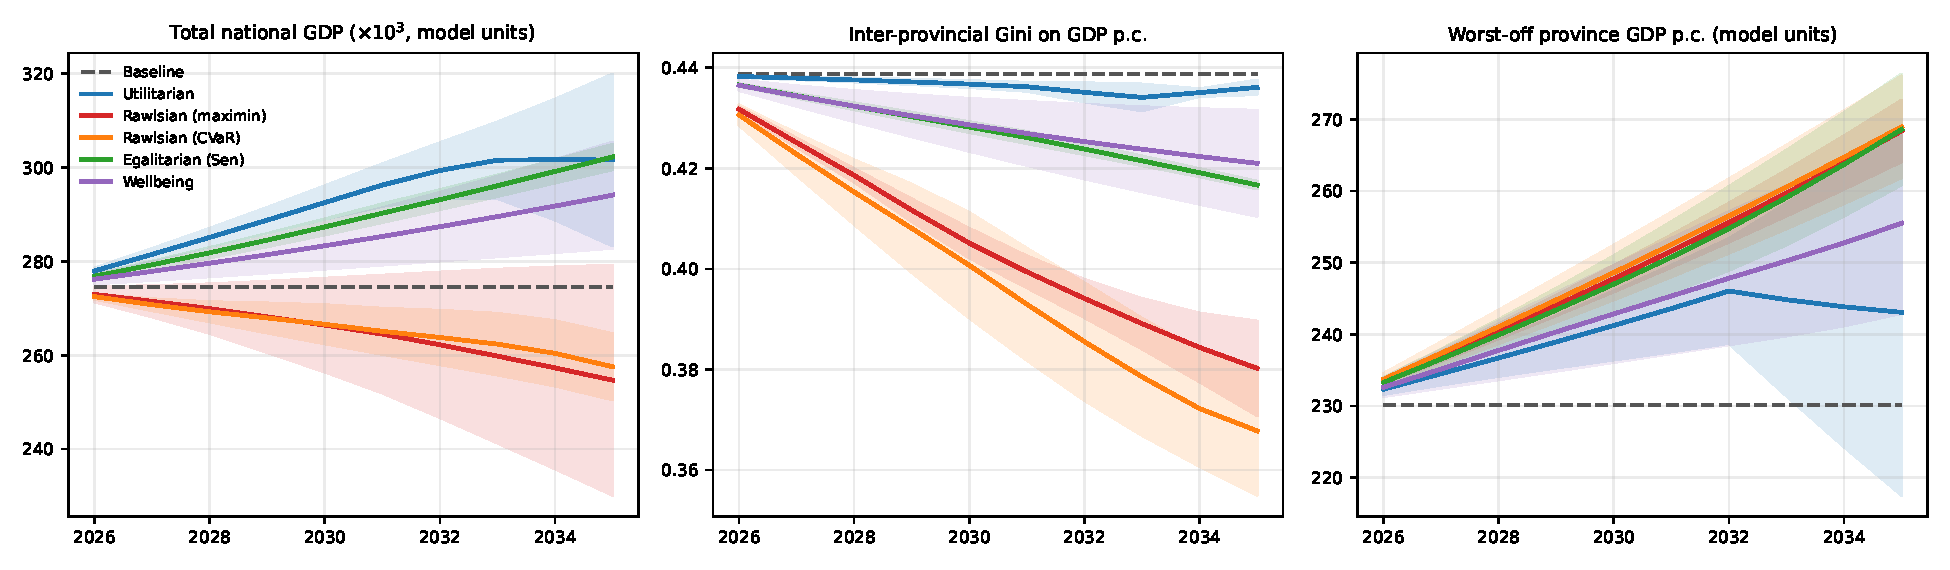
\includegraphics[width=\textwidth]{figures/trajectories.pdf}
\caption{Simulated trajectories 2026--\cmpFinalYear{} under each ethical
framework (same neural policy, same training budget, same budget constraint)
against the baseline scenario: total national GDP (left), inter-provincial
Gini on GDP per capita (center), worst-off province's GDP per capita (right).
Lines are the mean over \cmpSeeds{} seeds; shaded bands are $\pm1$ standard
deviation across seeds, i.e.\ the run-to-run spread of the gradient-free search.}
\label{fig:trajectories}
\end{figure}

Training improved the cumulative objective score over the untrained network by
\cmpUtilTrainImpr\% (utilitarian), \cmpRawlsTrainImpr\% (Rawlsian),
\cmpCvarTrainImpr\% (CVaR), \cmpEgalTrainImpr\% (egalitarian), and
\cmpWellTrainImpr\% (wellbeing), averaged over the \cmpSeeds{} seeds within the
six-iteration budget, the per-run training quality report that the model
card requires every optimization to disclose. Figure~\ref{fig:convergence}
plots the full convergence curves: how much of each framework's improvement is
already banked by iteration~6, and how the sparsest objective (hard maximin)
climbs slowest.

\begin{figure}[ht]
\centering
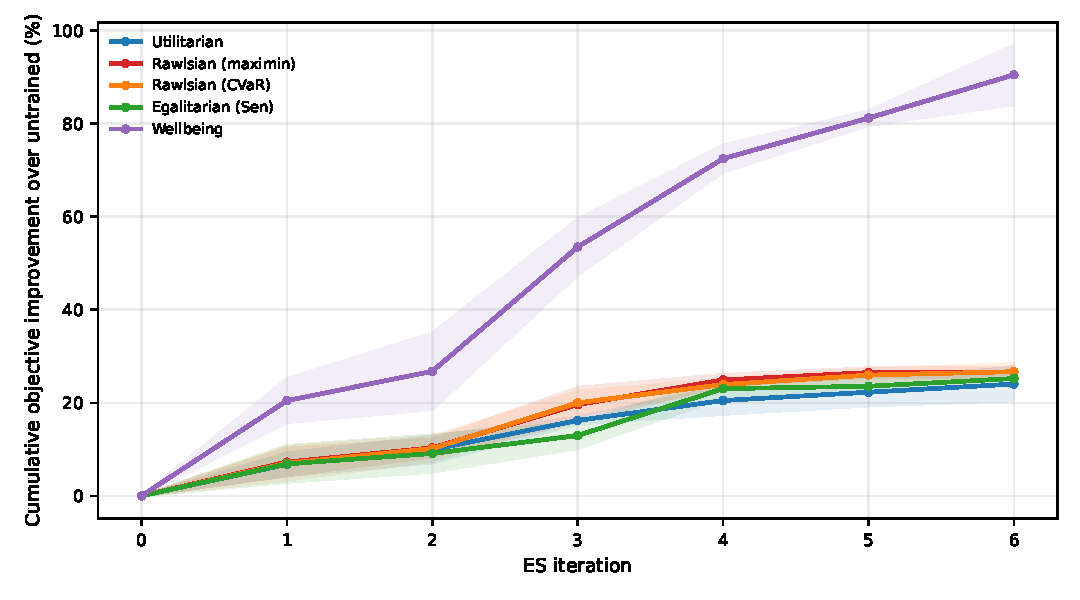
\includegraphics[width=0.74\textwidth]{figures/convergence.pdf}
\caption{Training convergence per framework: cumulative objective improvement
over the untrained network (\%) versus ES iteration, mean over \cmpSeeds{}
seeds (bands $\pm1$ std). Plotted as relative improvement so the four very
different objective scales are comparable on one axis. Hard maximin's
one-province signal gives it the least to climb on; the smoothed CVaR variant,
scoring the worst 20\% of provinces, gets a denser gradient.}
\label{fig:convergence}
\end{figure}

\subsection{Who gains, who loses}

Aggregates hide the distributional signature of each framework, which is the
ethically relevant part. Figure~\ref{fig:deltas} disaggregates the final year
to provinces: for each framework, the distribution over the 110 provinces of
the percent change in final-year GDP per capita relative to the baseline
scenario, the headless counterpart of the UI's ``who gains, who loses''
maps.

\begin{figure}[ht]
\centering
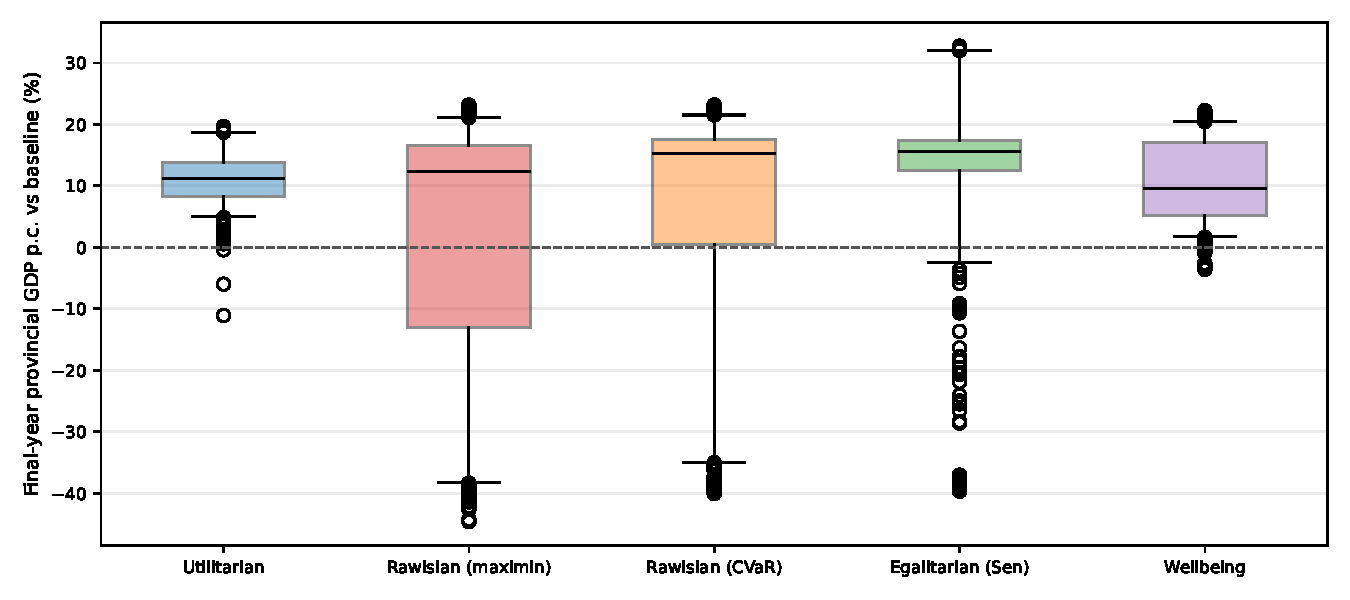
\includegraphics[width=0.82\textwidth]{figures/province_deltas.pdf}
\caption{Distribution over the 110 provinces of final-year GDP per capita
change versus the baseline scenario, per ethical framework (boxes: quartiles;
whiskers: 5th--95th percentile). The frameworks differ not only in their means
but in the \emph{shape} of who benefits.}
\label{fig:deltas}
\end{figure}

\subsection{The North--South divide}
\label{sec:northsouth}

The introduction chose Italy because of one cleavage in particular (the
North--South divide), yet the results so far speak only in province-agnostic
aggregates. This section reads them in the dimension that motivated the project.
The 110 provinces are grouped into Italy's standard statistical macro-areas
(\code{province\_mapping.PROVINCE\_TO\_MACROAREA}): the \nsProvNorth-province
North (Nord-Ovest + Nord-Est), the \nsProvCentre-province Centre, and the
\nsProvSouth-province South, or \emph{Mezzogiorno} (Sud + Isole). In the
starting state the South's mean provincial GDP per capita is \nsBaseSouth{}
against the North's \nsBaseNorth, a South/North ratio of \nsBaseRatio, the
divide the literature describes. Table~\ref{tab:northsouth} and
Figure~\ref{fig:northsouth} report what each framework does to it.

\begin{table}[ht]
\centering
\small
\begin{tabular}{lrrr}
\toprule
\textbf{Objective} & \textbf{North $\Delta$} & \textbf{South $\Delta$} &
\textbf{South/North ratio} \\
\midrule
Baseline & --- & --- & \nsBaseRatio \\
Utilitarian (total GDP) & \nsUtilNorth\% & \nsUtilSouth\% & \nsUtilRatio \\
Rawlsian (maximin) & \nsRawlsNorth\% & \nsRawlsSouth\% & \nsRawlsRatio \\
Rawlsian (CVaR) & \nsCvarNorth\% & \nsCvarSouth\% & \nsCvarRatio \\
Egalitarian (Sen) & \nsEgalNorth\% & \nsEgalSouth\% & \nsEgalRatio \\
Wellbeing & \nsWellNorth\% & \nsWellSouth\% & \nsWellRatio \\
\bottomrule
\end{tabular}
\caption{North vs South response by ethical framework: mean provincial GDP per
capita change from baseline for the North and the Mezzogiorno, and the resulting
South/North ratio (higher = a narrower divide; baseline \nsBaseRatio). Means
over \cmpSeeds{} seeds.}
\label{tab:northsouth}
\end{table}

\begin{figure}[ht]
\centering
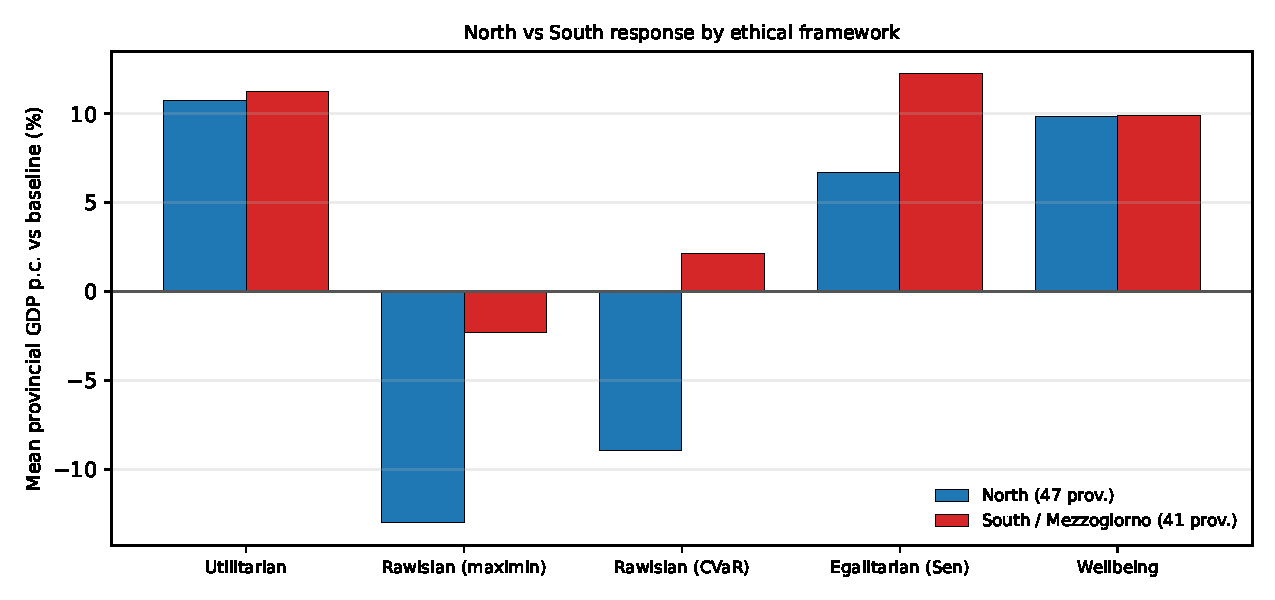
\includegraphics[width=0.82\textwidth]{figures/north_south.pdf}
\caption{North (blue) vs South/Mezzogiorno (red) mean provincial GDP per capita
change from baseline, per framework (\cmpSeeds-seed means). A taller red bar
than blue means the framework closes the divide by lifting the South; a deep
blue trough means it closes the divide by pulling the North down.}
\label{fig:northsouth}
\end{figure}

Four territorial signatures emerge, and they sharpen the abstract results:

\begin{itemize}
    \item \textbf{Utilitarianism and wellbeing leave the divide untouched.}
    Both lift North and South by almost exactly the same proportion
    (\nsUtilNorth\%/\nsUtilSouth\% and \nsWellNorth\%/\nsWellSouth\%), so the
    South/North ratio barely moves from baseline (\nsUtilRatio, \nsWellRatio
    vs.\ \nsBaseRatio). A distribution-blind rising tide raises the Mezzogiorno
    in step with the North, it neither closes nor widens the gap, it
    \emph{photocopies} it onto a richer Italy.
    \item \textbf{Maximin closes the divide by leveling the North down.}
    It produces the most equal territorial outcome of any framework
    (ratio \nsRawlsRatio), but the mechanism is the leveling-down objection
    in geographic form: the North \emph{falls} \nsRawlsNorth\% while the South
    barely moves (\nsRawlsSouth\%). The gap narrows because the top is cut, not
    because the bottom rises.
    \item \textbf{CVaR closes it more humanely.} The smoothed maximin reaches
    essentially the same ratio (\nsCvarRatio) but the South actually
    \emph{gains} (\nsCvarSouth\%) while the North falls less (\nsCvarNorth\%),
    a strictly kinder route to the same territorial equality, and the
    Mezzogiorno's only Rawlsian-family improvement.
    \item \textbf{Sen welfare is the cohesion result.} Egalitarianism is the
    one framework that narrows the divide (ratio \nsEgalRatio) \emph{while both
    regions grow}: it lifts the South faster than the North
    (\nsEgalSouth\% vs.\ \nsEgalNorth\%), the textbook definition of territorial
    cohesion, convergence without sacrifice.
\end{itemize}

Two honesty notes. First, the \emph{absolute} North--South gap in the twin is a
property of the disaggregated starting data (GDP is one of the regionally
disaggregated indicators; Section~\ref{sec:data}), so the numbers above are read
as each framework's \emph{change} to the gap within the simulator, not as a
measurement of Italy's real divide. Second, precisely because of that, the
macro-area average over \nsProvNorth--\nsProvSouth{} provinces is a
\emph{sounder} unit than the single worst-off province the headline metrics
lean on: aggregating washes out the per-province disaggregation noise, so the
territorial reading here is, if anything, more robust than the floor it
complements.

\subsection{The efficiency--equity frontier}

Figure~\ref{fig:pareto} shows the NSGA-II result: \parPoints{} non-dominated
uniform national policies from \parEvals{} twin rollouts. Across the front,
total GDP spans \parGdpSpanLo--\parGdpSpanHi{} ($\times 10^3$) and the
worst-off province's GDP per capita spans \parWorstLo--\parWorstHi{}, and
the two move together with correlation \parCorr{}, while the inter-provincial
Gini is invariant across the entire front to within
$\sim$\parGiniSpanMicro$\times 10^{-6}$ (at \parGiniLo{} everywhere, to three
decimals).

This degeneracy is the experiment's most instructive structural finding:
\emph{in the space of uniform national policies, there is no
efficiency--equity trade-off to map}. A single lever vector applied
identically to every province moves all provinces nearly proportionally in
the twin's multiplicative dynamics, a stronger national stance produces
more total GDP \emph{and} a higher floor in lockstep, and relative dispersion
barely responds. The expected three-cornered frontier collapses to a ray, and
the tagged ``corners'' pile onto its ends (the utilitarian and Rawlsian
corners coincide at the high end; the egalitarian tag lands on a point
distinguished only by Gini noise at the $10^{-6}$ scale). The genuine
distributional divergence seen in Table~\ref{tab:headline}, Gini moving
from 0.439 to \cmpRawlsGini{}, was produced by the \emph{per-province}
neural policy, which can treat provinces differently. The conclusion writes
itself: in this twin, equity is purchased by \emph{targeting}, not by the
overall level of the national policy stance; an ethical framework only has
distributional teeth if the policy class can discriminate between its moral
patients.

\begin{figure}[ht]
\centering
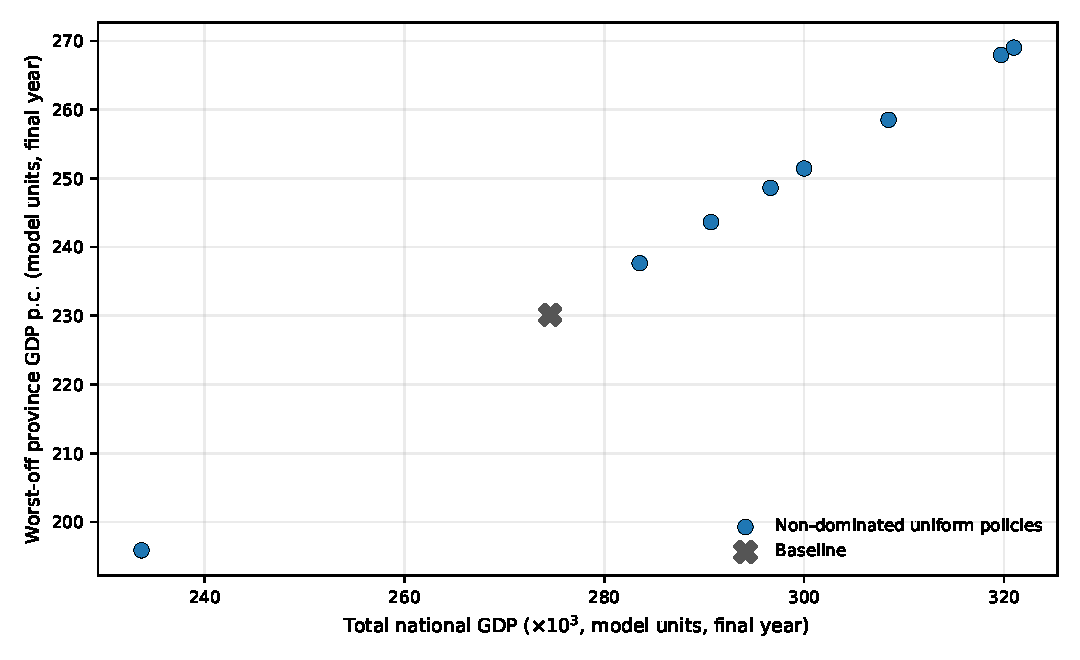
\includegraphics[width=0.76\textwidth]{figures/pareto.pdf}
\caption{The NSGA-II non-dominated set over uniform national lever vectors
(\parGens{} generations, population \parPop{}; final-year metrics), plotted as
efficiency versus the floor. The set degenerates to a ray: total GDP and the
worst-off province co-move (correlation \parCorr) and the Gini is invariant
to $\sim 10^{-6}$, so uniform national policy cannot trade efficiency against
equity, only per-province targeting can (Table~\ref{tab:headline}). The
gray cross marks the baseline scenario.}
\label{fig:pareto}
\end{figure}

\subsection{The frontier returns once policy can target: the clustered search}
\label{sec:clustered}

The uniform degeneracy predicts its own remedy: if equity is purchased by
targeting, then giving the Pareto search the \emph{ability} to target should
make inequality move. Re-running the identical NSGA-II over per-cluster lever
vectors, \parcClusters{} k-means regional packages instead of one national
vector, the same population and generation budget, does exactly that
(Figure~\ref{fig:paretoclustered}). The front is small (\parcPoints{}
non-dominated policies; an $80$-dimensional genome is under-resolved by
\parEvals{} rollouts), but it already does what the uniform front could not:
the inter-provincial Gini \emph{varies}, from \parcGiniLo{} to \parcGiniHi{}
across the front, against the uniform front's invariance to $10^{-6}$. The
mechanism is exactly the predicted one: the lowest-Gini policy holds the
richest cluster back while the highest-GDP policy feeds it. One nuance the
numbers insist on: total GDP and the \emph{floor} still co-move along the
clustered front (they rise together from the egalitarian to the utilitarian
corner), so what targeting opens is an efficiency-versus-\emph{inequality}
trade-off, not an efficiency-versus-floor one. That is the same lesson as
Table~\ref{tab:headline}, now isolated in a white-box, read-only search:
\emph{inequality responds to who is treated differently, not to how hard the
single national lever is pushed}. The regional packages remain fully
inspectable: each front point expands into one lever table per cluster, the
way a real ``plan for the Mezzogiorno'' would read.

\begin{figure}[ht]
\centering
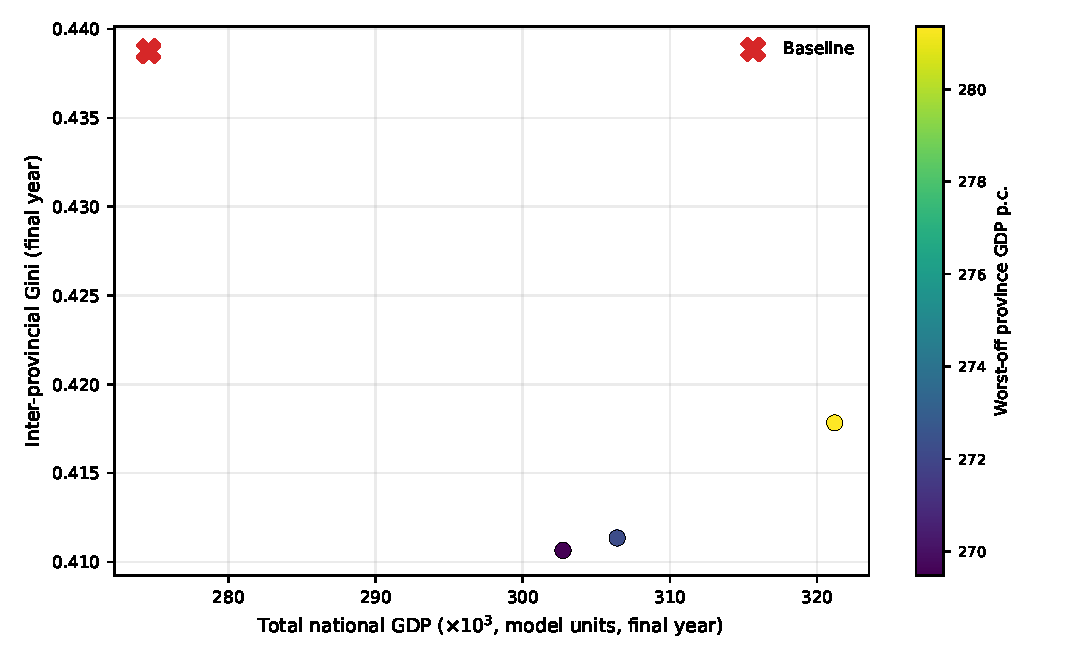
\includegraphics[width=0.78\textwidth]{figures/pareto_clustered.pdf}
\caption{NSGA-II over \emph{per-cluster} lever vectors (\parcClusters{} k-means
regional packages; \parGens{} generations, population \parPop{}). Unlike the
uniform front, this one spans a real range of inequality (Gini
\parcGiniLo--\parcGiniHi), so efficiency (horizontal) and equity (vertical) are
genuinely in tension; colour encodes the worst-off province's GDP. The red
cross marks the baseline. Targeting, not the overall intensity of national
policy, is what opens the trade-off.}
\label{fig:paretoclustered}
\end{figure}

\subsection{The prioritarian continuum, swept}
\label{sec:sweep}

The objectives so far are discrete points; the prioritarian objective
(Section~\ref{sec:notimplemented}) is instead a \emph{dial}. Its concavity
$\rho$ interpolates between utilitarian ($\rho{=}0$, identical by construction)
and maximin ($\rho{\to}1$), so sweeping it should trace the efficiency--floor
continuum that the uniform Pareto search could not. Training the neural policy
at a ladder of concavities (\sweepSeeds-seed means; Figure~\ref{fig:sweep})
confirms it: as $\rho$ rises from $0$ to \sweepRhoHi, total GDP moves from
\sweepGdpAtZero\% to \sweepGdpAtHi\% versus baseline while the worst-off
province rises from \sweepWorstAtZero\% to \sweepWorstAtHi\%, and the Gini falls
from \sweepGiniAtZero{} to \sweepGiniAtHi. The $\rho{=}0$ end reproduces the
utilitarian objective by construction; its sweep figures differ from the
headline utilitarian row of Table~\ref{tab:headline} only by seed noise (this
sweep averages \sweepSeeds{} seeds against the headline's \cmpSeeds{}, and the
floor is the highest-variance axis). A single scalar slides the optimizer
from the rising tide to the floor-first regime, the prioritarian gradient
that sits, philosophically and now empirically, between SERA's two endpoints,
and a concrete way for a decision-maker to choose \emph{how much} priority the
worst-off get rather than toggling between extremes.

\begin{figure}[ht]
\centering
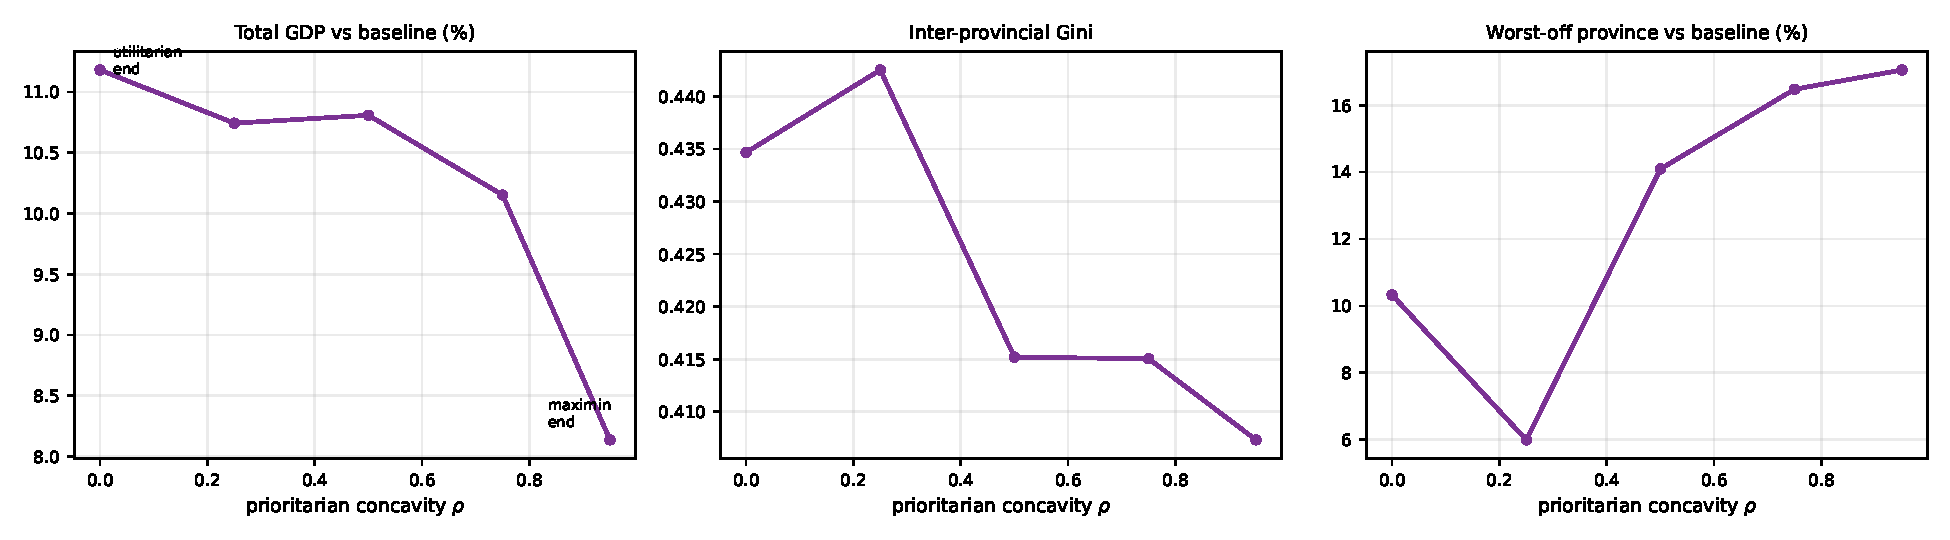
\includegraphics[width=\textwidth]{figures/prioritarian_sweep.pdf}
\caption{Prioritarian sweep: final-year total GDP (left), inter-provincial Gini
(center), and the worst-off province (right) as the concavity $\rho$ rises from
the utilitarian end ($\rho{=}0$) toward maximin. Means over \sweepSeeds{} seeds.
The single parameter traces the efficiency--equity continuum as a curve.}
\label{fig:sweep}
\end{figure}

\subsection{The sufficiency threshold, swept}
\label{sec:suffsweep}

The other tunable objective is sufficientarian: minimise the shortfall below a
threshold $\theta$, where everything above $\theta$ is morally irrelevant and
$\theta$ \emph{is} the theory (Section~\ref{sec:notimplemented}). Sweeping it
(\suffSeeds-seed means, $\theta$ as a multiple of the starting median province;
Figure~\ref{fig:suffsweep}) shows the optimizer responding to where the
``enough'' line is drawn, but not in the way one might first guess. As
$\theta$ rises from \suffThetaLo{} to \suffThetaHi{} the floor stays high
(\suffWorstAtLo\%~$\to$~\suffWorstAtHi\% over baseline) and inequality stays low
(Gini \suffGiniAtLo~$\to$~\suffGiniAtHi, well below the baseline \baseGini); what
moves sharply is the \emph{GDP cost}, from \suffGdpAtLo\% to \suffGdpAtHi\%. The
mechanism is instructive: a low bar marks only the very poorest as ``not
enough,'' which the optimizer meets with concentrated, costly transfers; a higher
bar implicates most provinces, which it meets with a broader and far cheaper
lift. Where the sufficiency line sits changes less about the floor reached than
about how much growth is sacrificed to hold it, the sufficientarian trade-off,
made selectable rather than smuggled into a default. That the threshold is exposed as a slider rather than a
hard-coded constant is the point: the one value that carries the entire moral
content of the framework is placed in the user's hands, not smuggled into a
default.

\begin{figure}[ht]
\centering
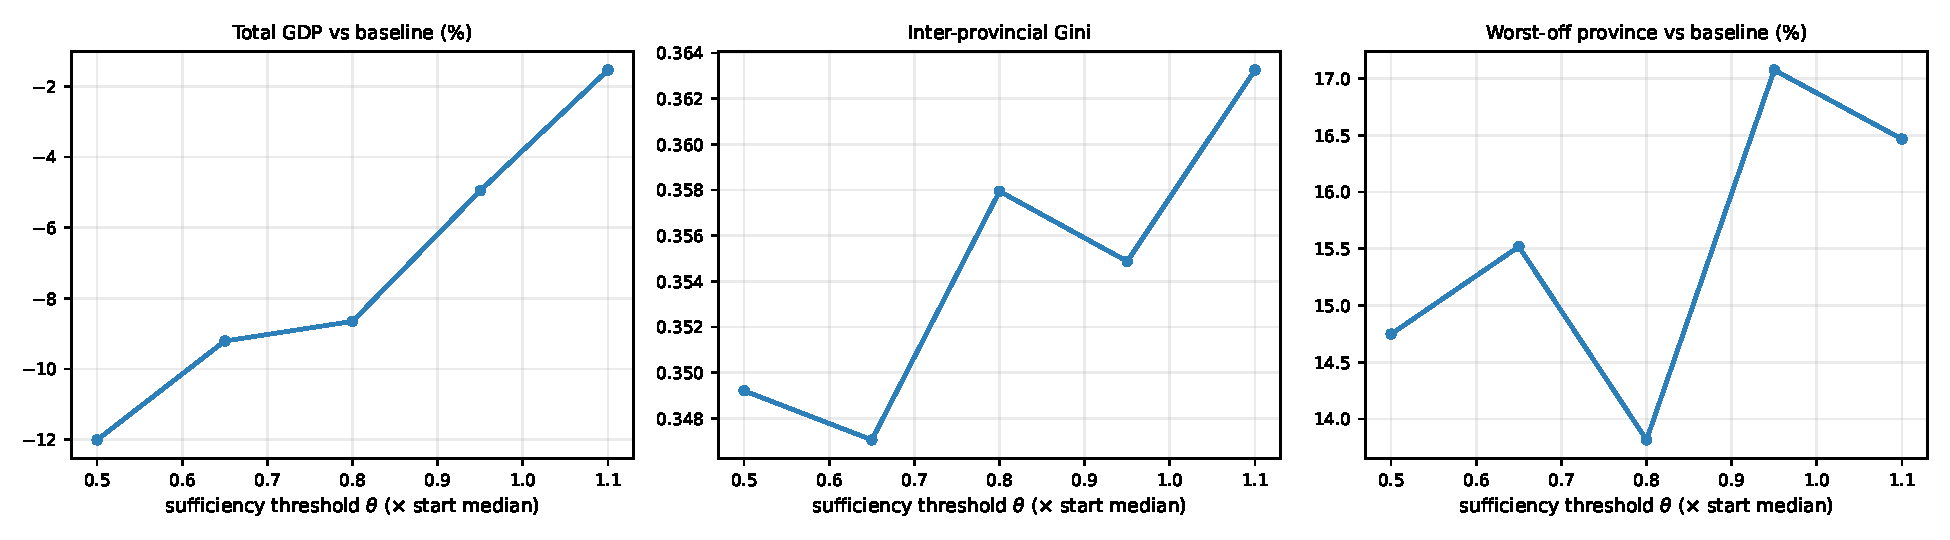
\includegraphics[width=\textwidth]{figures/sufficientarian_sweep.pdf}
\caption{Sufficientarian sweep: final-year total GDP (left), Gini (center), and
the worst-off province (right) as the sufficiency threshold $\theta$ rises.
Means over \suffSeeds{} seeds. Raising the ``enough'' line shifts the
optimizer's effort toward the floor.}
\label{fig:suffsweep}
\end{figure}

\subsection{How much the sign review matters: a propagation ablation}
\label{sec:ablation}

The inter-indicator propagation was changed twice in this work: from
sign-\emph{less} (every target moved with its source) to \emph{documented}
(polarity-derived signs), and then to \emph{reviewed} (those signs corrected by
the panel; Section~\ref{sec:datareview}). Table~\ref{tab:ablation} re-runs the
headline comparison (\ablSeeds{} seeds) under all three to show the change is
load-bearing, not cosmetic. The decisive step is making propagation
sign-\emph{aware} at all: moving from \code{signless} to \code{documented}
shifts the egalitarian floor and Gini materially, because mis-signed links like
income$\to$poverty were previously pushing inequality the wrong way. The panel
\code{review} on top, flipping \strEdgesFlipped{} edges and dropping
\strEdgesDropped{} unsupported ones, is a smaller, data-driven refinement.
The control column (utilitarian Gini, which should barely move since
utilitarianism is distribution-blind) stays nearly flat across modes, as
expected.

\begin{table}[ht]
\centering
\small
\begin{tabular}{lrrrr}
\toprule
\textbf{Propagation mode} & \textbf{Egal.\ floor} & \textbf{Egal.\ Gini} &
\textbf{Rawls floor} & \textbf{Util.\ Gini (control)} \\
\midrule
Sign-less (original) & \ablSignlessEgalWorst\% & \ablSignlessEgalGini & \ablSignlessRawlsWorst\% & \ablSignlessUtilGini \\
Documented signs & \ablDocumentedEgalWorst\% & \ablDocumentedEgalGini & \ablDocumentedRawlsWorst\% & \ablDocumentedUtilGini \\
Reviewed (ships) & \ablReviewedEgalWorst\% & \ablReviewedEgalGini & \ablReviewedRawlsWorst\% & \ablReviewedUtilGini \\
\bottomrule
\end{tabular}
\caption{Propagation-mode ablation (\ablSeeds{} seeds): floor change vs.\
baseline and final Gini under each inter-indicator propagation rule. Making
propagation sign-aware (sign-less $\to$ documented) is the load-bearing change;
the panel review is a smaller refinement on top. The utilitarian Gini is a
control and barely moves.}
\label{tab:ablation}
\end{table}

\subsection{The price of transparency, measured}
\label{sec:transparency}

Section~\ref{sec:policymodels} claims the explainability spectrum lets the
black-box-vs-white-box performance gap be \emph{measured} per problem rather
than assumed, but the comparison so far uses only the neural policy. Training
every model under one objective (utilitarian), one budget, and \transSeeds{}
seeds closes that gap (Table~\ref{tab:transparency},
Figure~\ref{fig:transparency}). The result is the encouraging one for
contestability: in this twin the white-box models pay little or nothing for
their legibility. The linear policy, the same per-province setup as the
neural one minus the hidden layer, scores \transLinearRel\% of the neural
policy's cumulative objective; the cross-entropy uniform and cluster policies and
the rule list land within a few percent of it too. More strikingly, the
gray-box Gaussian-process policy \emph{edges past} the black box
(\transUnifBayesRel\%), so here legibility is not merely cheap but, for one
model, free. With the twin's effects bounded by the realism caps, the extra
expressive capacity of a hidden layer buys little, and the inherently
interpretable models recover essentially all of it, the empirical half of
Rudin's argument~\cite{rudin2019}, answered with data for this problem instance
rather than asserted.

\begin{table}[ht]
\centering
\small
\begin{tabular}{llrrr}
\toprule
\textbf{Policy model} & \textbf{Badge} & \textbf{Score (\% of neural)} &
\textbf{Total GDP} & \textbf{Gini} \\
\midrule
Neural (MLP) & \transNeuralBadge & \transNeuralRel & \transNeuralGdp & \transNeuralGini \\
Linear & \transLinearBadge & \transLinearRel & \transLinearGdp & \transLinearGini \\
Rule list & \transRulesBadge & \transRulesRel & \transRulesGdp & \transRulesGini \\
Regional clusters & \transClusterBadge & \transClusterRel & \transClusterGdp & \transClusterGini \\
Uniform (CEM) & \transUnifCemBadge & \transUnifCemRel & \transUnifCemGdp & \transUnifCemGini \\
Uniform (Bayesian) & \transUnifBayesBadge & \transUnifBayesRel & \transUnifBayesGdp & \transUnifBayesGini \\
\bottomrule
\end{tabular}
\caption{Price of transparency (\transSeeds{} seeds, utilitarian objective):
each policy model's cumulative objective score as a percentage of the neural
policy's, with its explainability badge and final-year metrics. The white-box
models recover most of the black box's performance, so transparency is cheap in
this twin.}
\label{tab:transparency}
\end{table}

\begin{figure}[ht]
\centering
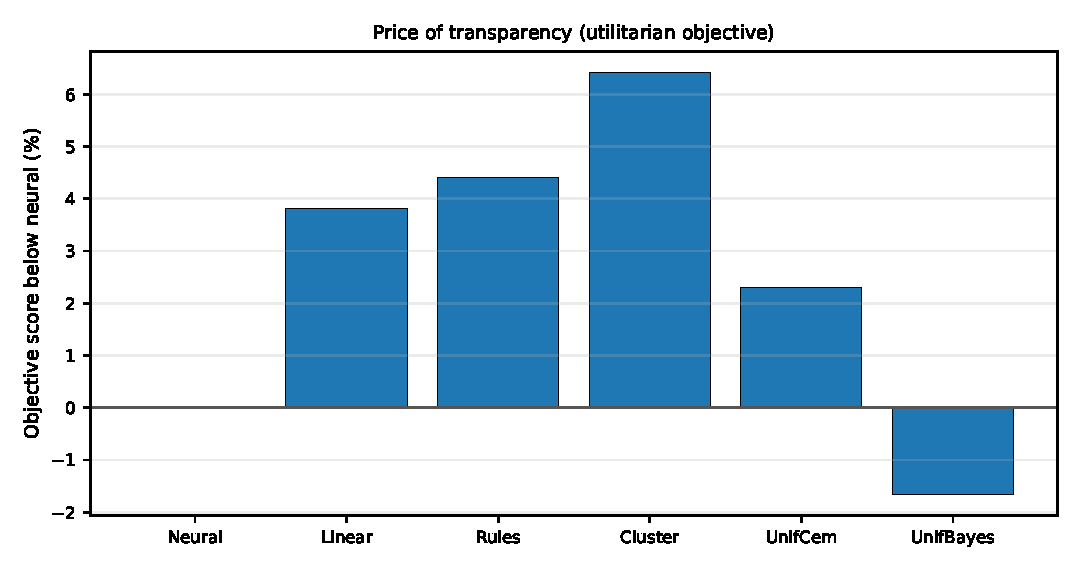
\includegraphics[width=0.7\textwidth]{figures/transparency.pdf}
\caption{The score gap to the neural policy for each model (utilitarian
objective, \transSeeds{} seeds). Shorter bars are cheaper transparency; the
white-box models give up little.}
\label{fig:transparency}
\end{figure}

\subsection{Reading the results}

Six observations, with the standing caveat that they describe the simulator
(Section~\ref{sec:uncertainty}) and are means over \cmpSeeds{} seeds:

\begin{enumerate}
    \item \textbf{The frameworks genuinely diverge.} With the model, data,
    budget, and search budget held fixed, swapping the per-year welfare
    function alone produces measurably different futures on all three
    evaluation axes (Table~\ref{tab:headline}): total GDP ranges from
    \cmpRawlsGdpDelta\% (maximin) to \cmpUtilGdpDelta\% (utilitarian) versus
    baseline, the Gini from \cmpCvarGini{} to \cmpWellGini{}, and the floor from
    \cmpUtilWorstDelta\% to \cmpEgalWorstDelta\%. With \cmpSeeds{} seeds these
    carry tight bootstrap confidence intervals: the utilitarian GDP gain is
    \cmpUtilGdpDelta$\pm$\cmpUtilGdpCI\%, its floor \cmpUtilWorstDelta$\pm$%
    \cmpUtilWorstCI\% (95\% CI), and the headline orderings below that we
    flag as robust are exactly those whose intervals do not overlap. The ethical
    choice is not decorative: it is the difference between the rows.
    \item \textbf{The utilitarian optimum is a rising tide that under-serves the
    floor.} Utilitarianism grows total GDP the most (\cmpUtilGdpDelta\%) and
    leaves the Gini near baseline (\cmpUtilGini{} vs.\ \baseGini): the twin's
    multiplicative, capped dynamics make the sum-maximizer lift nearly every
    province by a similar amount (Figure~\ref{fig:deltas}, a tight box around
    $+11\%$). But distribution-blindness shows where it counts: the floor it
    reaches ($+$\cmpUtilWorstDelta\%) is the \emph{lowest} of the interventions
    and more seed-variable than the maximin-family floors
    ($\pm$\cmpUtilWorstStd{} on the worst-off province vs.\
    $\pm$\cmpRawlsWorstStd{} for maximin and $\pm$\cmpCvarWorstStd{} for CVaR).
    The rising tide does lift the floor, but only incidentally, and the
    frameworks that \emph{target} it reach $8$--$10$ points higher (below). The
    classic objection survives, in a milder form than the textbook: not
    sacrifice of the few, but indifference, the worst-off rise as a
    by-product rather than a goal.
    \item \textbf{Maximin reliably raises the floor, and multi-seed
    replication is what shows it.} Under \cmpSeeds{} seeds, maximin lifts the
    worst-off province by \cmpRawlsWorstDelta\% (to \cmpRawlsWorst) with one of
    the \emph{lowest} floor-variances of any framework ($\pm$\cmpRawlsWorstStd,
    second only to its smoothed CVaR variant below),
    comfortably above the utilitarian floor, the difference principle doing
    what it promises. This is worth dwelling on methodologically: a
    \emph{single}-seed version of this same experiment had shown maximin's
    floor landing fractionally \emph{below} the utilitarian one, which invited
    a tidy ``maximin under-optimizes its own objective'' story; replication
    dissolves that story as seed luck (the utilitarian floor's huge variance is
    what produced the crossing). It is a small but clean demonstration of why
    the multi-seed protocol of Section~\ref{sec:threats} matters: the headline
    of a gradient-free comparison can invert between seeds. What \emph{is}
    robust across seeds is the leveling-down \emph{shape}: maximin still cuts
    the richest tail hard (down roughly 35--45\% in Figure~\ref{fig:deltas})
    because everything above the minimum is worth nothing to it, and the GDP
    it concedes for the higher floor is a real \cmpRawlsGdpDelta\%.
    \item \textbf{Smoothing maximin weakly dominates it, answering the
    sparsity question.} The CVaR objective, scoring the worst 20\% of provinces
    instead of the single poorest, was included to test whether maximin's sparse
    one-province signal was the real source of its troubles. Across \cmpSeeds{}
    seeds CVaR matches or beats hard maximin on every axis of the means: an
    equal-or-higher floor (\cmpCvarWorst{} vs \cmpRawlsWorst), less GDP forgone
    (\cmpCvarGdpDelta\% vs \cmpRawlsGdpDelta\%), lower run-to-run variance, and
    the \emph{lowest Gini of any framework} (\cmpCvarGini). The honest reading,
    given the spreads: the \emph{floor} difference between the two is
    \sigCvarRawlsFloor{} (the paired 95\% bootstrap CI on the per-seed difference
    includes zero, they reach statistically the same floor), so smoothing the
    sparse signal does
    not \emph{cost} the floor; what it robustly buys is a lower GDP price, tighter
    inequality, and less seed variance. That is still a clean answer to the
    sparsity question, broadening maximin's signal to the bottom quintile is a
    free lunch on every axis except the floor it leaves untouched, and a
    concrete argument for preferring the CVaR form in practice.
    \item \textbf{Sen welfare is the efficiency--equity sweet spot.} The
    egalitarian run reaches the \emph{highest floor of any framework}
    (\cmpEgalWorstDelta\%, though at the \emph{largest} floor-variance of any
    framework, $\pm$\cmpEgalWorstStd)
    \emph{and} still grows total GDP (\cmpEgalGdpDelta\%), holding the Gini at
    \cmpEgalGini{}, achieved (Figure~\ref{fig:deltas}) by lifting almost
    every province while trimming only a handful of the richest. Because its
    score multiplies growth by equality, it draws training signal from the whole
    distribution, which is plausibly why it alone pairs the top floor with
    positive growth. Its floor advantage over the utilitarian run is
    \sigEgalUtilFloor{} across \cmpSeeds{} seeds (paired 95\% bootstrap CI). The wellbeing run lands with the utilitarian on GDP
    (\cmpWellGdpDelta\%) but distributes its gains tightly across every province,
    routed through its health/employment/poverty channels rather than GDP alone.
    \item \textbf{The frontier exposes where the trade-off actually lives.}
    The uniform-lever Pareto search finds \emph{no} efficiency--equity
    trade-off, efficiency and the floor co-move at correlation \parCorr{}
    and the Gini is flat to $10^{-6}$ (Figure~\ref{fig:pareto}). Giving the
    same search per-cluster levers (Figure~\ref{fig:paretoclustered}) makes the
    Gini vary for the first time (\parcGiniLo--\parcGiniHi), modest, and on
    an admittedly under-resolved front of \parcPoints{} points, but
    \emph{qualitatively absent} from the uniform run. Tellingly, GDP and the
    floor still co-move even on the clustered front: what targeting opens is an
    efficiency-versus-\emph{inequality} trade (hold back the richest cluster
    for a lower Gini), not an efficiency-versus-floor one. Equity, in this
    twin, is purchased by \emph{targeting}, not by the national policy level.
    For decision support the implication is concrete: ``how interventionist
    should national policy be?'' is the wrong equity question; ``who gets
    treated differently?'' is the right one, and that is precisely what the
    contestability machinery (Section~\ref{sec:explain}) exists to make
    auditable.
\end{enumerate}

Two structural qualifications. First, the effect sizes are bounded by design:
the policy-signal cap, the causal-rule strength, and the $\pm6\%$/year realism
cap mean that ten simulated years cannot diverge arbitrarily, so the
inter-framework differences are modest in absolute terms, which is
realistic for a decade of fiscal policy, and a direct consequence of the
calibration discussed in Section~\ref{sec:discussion}. Second, the ES training
budget (6 iterations) is the UI's interactive default, not a converged
optimum, and \cmpSeeds{} seeds tighten but do not eliminate run-to-run noise
(the standard deviations in the text are non-trivial); each row should be read
as ``what this framework finds with the standard interactive budget, averaged
over a handful of seeds,'' not as its global optimum.

\section{Discussion}
\label{sec:discussion}

\subsection{What the comparison shows}

The experiment of Section~\ref{sec:results} closes the loop the architecture
promises: with everything held fixed except the per-year welfare function, the
same optimizer is pulled to measurably different futures, and the frameworks'
\emph{relative signatures} are exactly as the theories say: maximin and its
CVaR cousin reliably raise the floor while cutting the richest tail, Sen
welfare reaches the highest floor of all while still growing, the wellbeing
composite reroutes gains through non-GDP channels, and the distribution-blind
utilitarian run grows the average the most while leaving the worst-off lowest
and more seed-variable than the frameworks that target it. Two lessons
generalize beyond the numbers. The first is methodological and was bought
precisely by the multi-seed protocol: a \emph{single}-seed version of this
experiment had maximin's floor landing below the utilitarian one, a tidy,
publishable ``maximin under-optimizes its own objective'' story that
\emph{evaporated under replication} as the utilitarian floor's large variance,
a cautionary tale about reading a gradient-free optimizer's headline off one
run. The second is substantive: a moral principle's practical meaning depends
on the response structure of the system it optimizes \emph{and} on how
optimizable its objective is, which is why we added the smoothed CVaR
maximin, and why the lesson it teaches (broadening maximin's one-province
signal to the bottom quintile improves the growth and inequality it delivers at
no cost to the floor) could only be read off an experiment that held the
theory fixed. The methodological content is the point: \emph{the moral
criterion is an experimental variable}, and a system built this way can answer
``what would the Rawlsian recommendation cost, and who pays?'' with a number, a
spread, and a map instead of a position paper.

\subsection{Trade-offs exist only under calibrated scarcity}

An engineering finding that is an ethical finding in disguise: with looser
caps (e.g., a policy-signal cap of 0.5 instead of 0.03) every intervention
saturates the $\pm6\%$ growth limit and all growth-favoring objectives collapse
onto the same optimum, the ethical comparison becomes vacuously flat. The
frameworks differentiate only because the budget constraint and the effect
caps force genuine choices. Distributive justice presupposes scarcity, in the
model exactly as in philosophy; a simulator that lets every policy succeed
everywhere has abolished the subject matter.

\subsection{The assumptions dominate aggressive scenarios}

Since the ML layer's relative response saturates its cap, the differentiated
structure of \emph{which} levers move \emph{which} indicators comes mostly
from the hand-written causal rules. The sensitivity band exists precisely
because of this: it shows, per run, how much of the projection rests on those
hand-tuned assumptions. The honest reading of Section~\ref{sec:results} is
therefore: the \emph{direction} and \emph{ordering} of the inter-framework
differences are meaningful (they follow from the objectives' mathematics
interacting with documented causal structure); the \emph{magnitudes} are
hostage to constants a domain expert wrote down.

\subsection{Threats to validity}
\label{sec:threats}

Beyond the simulator-versus-reality category error (stated throughout), three
internal threats deserve note. (i) \emph{Search noise and signal sparsity}:
gradient-free training with small budgets has run-to-run variance. The results
above already mitigate this by replicating every framework over \cmpSeeds{}
seeds and reporting mean $\pm$ standard deviation (the bands in
Figure~\ref{fig:trajectories}); the framework \emph{ordering} is stable across
seeds where the bands do not overlap, but a few-seed sample still cannot fully
pin the magnitudes, and more seeds would tighten them further. The objectives
also differ in how much training signal they emit per rollout: maximin
scores one province in 110, Sen welfare the whole distribution, which is
exactly why the smoothed CVaR objective is included: it isolates that
asymmetry by holding the Rawlsian \emph{theory} fixed while scoring the worst
20\% of provinces, so the gap between the \code{rawlsian} and \code{cvar} rows
of Table~\ref{tab:headline} is a direct, in-experiment estimate of how much of
hard maximin's poor floor is optimization difficulty rather than the
difference principle itself. (ii) \emph{Objective scale effects}: the objectives have
different score scales, and although each optimizer only compares candidates
within one objective, ES step-size interacts with score curvature, so
frameworks may be optimized with effectively different aggressiveness (the
wellbeing run's large relative training improvement, \cmpWellTrainImpr\%, is
mostly an artifact of its near-zero starting score). (iii) \emph{Proxy
leakage}: all three evaluation axes are GDP-denominated, which understates
what the wellbeing framework achieves on its own currency (health,
employment, poverty), its row in Table~\ref{tab:headline} is scored in a
currency it deliberately deprioritizes.

\subsection{Limits of the paradigm}

Finally, the optimization paradigm itself has ethical limits that no objective
choice cures. Relational equality (Section~\ref{sec:theory}) resists encoding
as a function over indicator vectors. Procedural justice (legitimacy,
participation, consent) is invisible to end-state scoring. People missing
from official statistics are missing from every objective
(Section~\ref{sec:data}). And the unit-of-fairness choice (the province)
hides all within-province distribution. SERA's contribution is not to solve
these but to keep them written on the box.

\section{Conclusions}
\label{sec:conclusions}

SERA demonstrates, end to end, what it takes to put an explicit ethical
governance layer around an AI optimizer that advises on public-resource
allocation. The central design move is separation of concerns: the world
model, the search procedure, and the moral criterion are three independent,
swappable components, so the value judgment is forced out of the code and into
a visible, user-facing choice. Around that core, the project assembles the
scaffolding responsible deployment would demand, an explainability spectrum
with a measured price of transparency, post-hoc audits that state their own
fidelity, sensitivity bands that quantify how much rests on assumptions, a
human-in-the-loop candidate/adopt workflow, and the
model-card/datasheet/ethics documentation triplet mapped onto the EU AI Act's
high-risk obligations.

The experimental comparison supports the project's framing claim: there is
no single ``correct'' ethical algorithm for resource allocation, and
sharpens it in two ways the design did not anticipate. First, a moral
principle's practical meaning depends both on the dynamics it optimizes and on
how readily it can be optimized: maximin and its smoothed CVaR variant
reliably protected the worst-off province (at a modest GDP cost and by visibly
sacrificing the richest tail), while the distribution-blind utilitarian run
grew the average most but left the floor lowest and more seed-variable than the
maximin-family frameworks that target it.
That last comparison only became trustworthy under replication: a single seed
had shown maximin's floor falling \emph{below} the utilitarian one, a tidy
``maximin under-optimizes itself'' story that multi-seed replication exposed as
search luck. The methodological moral is as durable as the philosophical one:
the headline of a gradient-free ethical comparison can invert between seeds, so
replication is not optional housekeeping but part of the claim. Second, the locus of the ethical choice is not where the
dropdown suggests: uniform national policy moved efficiency and the floor in
lockstep with inequality untouched, so the entire distributional question
lives in per-province targeting, exactly the part of a policy that
contestability machinery must make auditable. What an ethically serious
system can do is not resolve the choice of framework but \emph{refuse to make
it silently}, presenting trade-offs to be inspected, with every
candidate's reasoning auditable and every assumption priced.

The honest limitations are equally part of the conclusion: the twin's causal
core is hand-written and dominates aggressive scenarios; the experimental
magnitudes are bounded by calibrated caps; the data measure only the measured
population; and the unit of fairness is the province. A system that knows and
says what it cannot see is the difference between decision support and
automation bias with extra steps. Future work follows directly: a
user-thresholded sufficientarian objective and a concavity-parameterized
prioritarian one (Section~\ref{sec:notimplemented}), multi-seed replication of
the framework comparison, population-weighted welfare variants, and
within-province distribution if data permits.

\section{Reproducibility}
\label{sec:repro}

The project requires Python 3.11 and Node.js. From the repository root:

{\footnotesize
\begin{verbatim}
python -m venv .venv
.venv\Scripts\activate          # Windows (macOS/Linux: source .venv/bin/activate)
pip install -r requirements.txt
\end{verbatim}
}

Download the data (rate-limited; the full set is slow), train the twin, and run
the tests:

{\footnotesize
\begin{verbatim}
$env:PYTHONPATH = "$pwd\src"
python src/sera/downloader.py --indicator all
python -m sera.twin.cli --mode train-and-simulate --model-type ridge --sim-years 5
python -m pytest tests -q
\end{verbatim}
}

This writes \code{twin\_models.joblib} (used by the UI) and
\code{simulation\_results.csv}. The experiments of Section~\ref{sec:results}
are reproduced by (matplotlib required for the figures):

{\footnotesize
\begin{verbatim}
.venv\Scripts\python.exe report\run_experiments.py        # headline comparison + Pareto
.venv\Scripts\python.exe report\run_prioritarian_sweep.py # the continuum sweep
.venv\Scripts\python.exe report\run_ablation.py           # propagation-mode ablation
.venv\Scripts\python.exe report\run_transparency.py       # price of transparency
.venv\Scripts\python.exe report\run_sufficientarian_sweep.py  # sufficiency-threshold sweep
.venv\Scripts\python.exe report\plot_results.py           # figures + results_macros.tex
\end{verbatim}
}

which write the raw JSON to \code{report/results/}, the figures to
\code{report/figures/}, and every number quoted in this report to
\code{report/results\_macros.tex}. Then launch the control room:

\begin{verbatim}
cd ui
npm install
npm start
\end{verbatim}

The UI exposes the policy-model and ethical-objective dropdowns in the header,
the per-province allocators and budget meter, the optimizer with its three
candidates and sensitivity band, the \code{compare-objectives} equity
dashboard, and the \code{pareto-front} efficiency--equity frontier. The app
makes no network requests at runtime; raw ISTAT data is not redistributed and
is fetched by each user under ISTAT's terms.

\begin{thebibliography}{99}

\bibitem{bentham1789} Jeremy Bentham. \emph{An Introduction to the Principles
of Morals and Legislation}. London, 1789.

\bibitem{mill1863} John Stuart Mill. \emph{Utilitarianism}. London, 1863.

\bibitem{mulgan2007} Tim Mulgan. \emph{Understanding Utilitarianism}. Acumen
Publishing, Chesham, UK, 2007.

\bibitem{crisp1997} Roger Crisp. \emph{Mill on Utilitarianism}. Routledge
Philosophy Guidebooks. Routledge, 1997.

\bibitem{rawls1971} John Rawls. \emph{A Theory of Justice}. Harvard University
Press, 1971.

\bibitem{rawls2001} John Rawls. \emph{Justice as Fairness: A Restatement}.
Edited by Erin Kelly. Harvard University Press, 2001.

\bibitem{wenar2025} Leif Wenar. ``John Rawls.'' In \emph{The Stanford
Encyclopedia of Philosophy}, edited by Edward N. Zalta and Uri Nodelman.
Metaphysics Research Lab, Stanford University, 2025.

\bibitem{harsanyi1975} John C. Harsanyi. ``Can the Maximin Principle Serve as
a Basis for Morality? A Critique of John Rawls's Theory.'' \emph{American
Political Science Review} 69(2):594--606, 1975.

\bibitem{bidadanure2025} Juliana Bidadanure and David Axelsen.
``Egalitarianism.'' In \emph{The Stanford Encyclopedia of Philosophy}, edited
by Edward N. Zalta and Uri Nodelman. Metaphysics Research Lab, Stanford
University, 2025.

\bibitem{lamont2017} Julian Lamont and Christi Favor. ``Distributive
Justice.'' In \emph{The Stanford Encyclopedia of Philosophy}, edited by Edward
N. Zalta. Metaphysics Research Lab, Stanford University, 2017.

\bibitem{anderson1999} Elizabeth S. Anderson. ``What Is the Point of
Equality?'' \emph{Ethics} 109(2):287--337, 1999.

\bibitem{sen1980} Amartya Sen. ``Equality of What?'' In \emph{Tanner Lectures
on Human Values}, Vol.~1. Cambridge University Press, 1980.

\bibitem{sen1976} Amartya Sen. ``Real National Income.'' \emph{The Review of
Economic Studies} 43(1):19--39, 1976.

\bibitem{frankfurt1987} Harry Frankfurt. ``Equality as a Moral Ideal.''
\emph{Ethics} 98(1):21--43, 1987.

\bibitem{timmer2021} Dick Timmer. ``Sufficientarianism.'' \emph{Philosophy
Compass} 16(7):e12755, 2021.

\bibitem{parfit1997} Derek Parfit. ``Equality and Priority.'' \emph{Ratio}
10(3):202--221, 1997.

\bibitem{stiglitz2009} Joseph E. Stiglitz, Amartya Sen, and Jean-Paul
Fitoussi. \emph{Report by the Commission on the Measurement of Economic
Performance and Social Progress}. Paris, 2009.

\bibitem{moor2006} James H. Moor. ``The Nature, Importance, and Difficulty of
Machine Ethics.'' \emph{IEEE Intelligent Systems} 21(4):18--21, 2006.

\bibitem{jobin2019} Anna Jobin, Marcello Ienca, and Effy Vayena. ``The global
landscape of AI ethics guidelines.'' \emph{Nature Machine Intelligence}
1:389--399, 2019.

\bibitem{rudin2019} Cynthia Rudin. ``Stop explaining black box machine
learning models for high stakes decisions and use interpretable models
instead.'' \emph{Nature Machine Intelligence} 1(5):206--215, 2019.

\bibitem{mitchell2019} Margaret Mitchell et al. ``Model Cards for Model
Reporting.'' In \emph{Proceedings of the Conference on Fairness,
Accountability, and Transparency (FAT*)}, pp. 220--229, 2019.

\bibitem{gebru2021} Timnit Gebru et al. ``Datasheets for Datasets.''
\emph{Communications of the ACM} 64(12):86--92, 2021.

\bibitem{deb2002} Kalyanmoy Deb, Amrit Pratap, Sameer Agarwal, and T.
Meyarivan. ``A fast and elitist multiobjective genetic algorithm: NSGA-II.''
\emph{IEEE Transactions on Evolutionary Computation} 6(2):182--197, 2002.

\bibitem{salimans2017} Tim Salimans, Jonathan Ho, Xi Chen, Szymon Sidor, and
Ilya Sutskever. ``Evolution Strategies as a Scalable Alternative to
Reinforcement Learning.'' arXiv:1703.03864, 2017.

\bibitem{rubinstein2004} Reuven Y. Rubinstein and Dirk P. Kroese. \emph{The
Cross-Entropy Method: A Unified Approach to Combinatorial Optimization,
Monte-Carlo Simulation and Machine Learning}. Springer, 2004.

\bibitem{frazier2018} Peter I. Frazier. ``A Tutorial on Bayesian
Optimization.'' arXiv:1807.02811, 2018.

\bibitem{aiact2024} European Parliament and Council. \emph{Regulation (EU)
2024/1689 laying down harmonised rules on artificial intelligence (Artificial
Intelligence Act)}. Official Journal of the European Union, 2024.

\end{thebibliography}

\appendix

\section{Implementation Algorithms}

Since the algorithms are central to how the ethical objectives act on the
system, the main ones are listed here for reference.

\begin{algorithm}[ht]
\caption{One simulated year (\code{DigitalTwinSimulator.simulate\_year})}
\label{alg:simyear}
\KwData{state $s_t$ (110 provinces $\times$ indicators), levers $a_t$,
trained models $\{f_k\}$, caps $\kappa_{\text{sig}}{=}0.03$,
$\kappa_{\text{rule}}{=}0.02$, $g_{\max}{=}0.06$}
\KwResult{next-year state $s_{t+1}$}
\ForEach{indicator $k$, province $p$}{
    $\hat{y} \leftarrow f_k(\text{lagged indicators}, a_t)$;\quad
    $\hat{y}_0 \leftarrow f_k(\text{lagged indicators}, a_{\text{baseline}})$\;
    $\delta \leftarrow \mathrm{clip}\!\big((\hat{y} - \hat{y}_0)/|y_{t}|,\,
    -\kappa_{\text{sig}},\, \kappa_{\text{sig}}\big)$
    \tcp*{anchored: only the policy signal is trusted}
    $y' \leftarrow y_t \cdot (1 + \delta)$\;
    \ForEach{lever $\ell$ with a causal edge $\ell \to k$}{
        $\sigma \leftarrow \tanh\!\big((a_{t,\ell} - \text{median}_\ell)/
        \text{scale}_\ell\big)$
        \tcp*{historical normalization}
        $y' \leftarrow y' \cdot \big(1 + \kappa_{\text{rule}} \cdot \sigma
        \cdot \mathrm{dir}(\ell, k)\big)$\;
    }
}
propagate inter-indicator effects along the dependency graph (dampened)\;
clip each indicator to its logical bounds\;
cap year-over-year change at $\pm g_{\max}$ per indicator
\tcp*{realism speed limit}
\Return $s_{t+1}$\;
\end{algorithm}

\begin{algorithm}[ht]
\caption{National budget constraint (applied every simulated year)}
\label{alg:budget}
\KwData{allocations $a$, state $s$, reserve $r$, spending intensity $\beta$}
\KwResult{feasible allocations $a'$, new reserve $r'$}
$\text{pool} \leftarrow \beta \cdot \mathrm{GDP}(s) \cdot
\overline{\big(a_{\tau} / a_{\tau}^{\text{base}}\big)}_{\tau \in \text{tax levers}}$
\tcp*{tax cuts below baseline shrink the pool}
$\text{cost} \leftarrow \sum_{p}\sum_{\ell \in \text{spending}}
\text{cost}\big(a_{p,\ell}\big)$\;
\eIf{$\text{cost} > \text{pool} + r$}{
    scale all spending levers down by $(\text{pool}+r)/\text{cost}$
    toward baseline\;
}{
    leave allocations unchanged\;
}
$r' \leftarrow \max\big(0,\; r + \text{pool} - \min(\text{cost},\,
\text{pool}+r)\big)$
\tcp*{unspent budget carries over}
\Return $(a', r')$\;
\end{algorithm}

\begin{algorithm}[ht]
\caption{Mirrored-sampling Evolution Strategies
(\code{neural} and \code{linear} policies)}
\label{alg:es}
\KwData{evaluate $J(\theta)$ (cumulative ethical welfare,
Eq.~\ref{eq:cumwelfare}), init $\theta_0$, popsize $N{=}6$, noise
$\sigma{=}0.25$, step $\alpha{=}0.2$}
$(\theta^\ast, J^\ast) \leftarrow (\theta_0, J(\theta_0))$\;
\For{$i = 1 \dots \text{iterations}$}{
    sample $\varepsilon_1, \dots, \varepsilon_N \sim \mathcal{N}(0, I)$;\quad
    evaluate $J$ at $\theta \pm \sigma\varepsilon_j$ (2$N$ rollouts,
    mirrored)\;
    normalize scores to advantages $A$ (zero mean, unit variance)\;
    $g \leftarrow \frac{1}{2N\sigma} \sum_j A_j \,\varepsilon_j^{(\pm)}$
    \tcp*{ES gradient estimate}
    $\theta \leftarrow \theta + \alpha g$;\quad
    update $(\theta^\ast, J^\ast)$ if any candidate improved\;
}
\Return $\theta^\ast$
\tcp*{best evaluated weights, not the last center}
\end{algorithm}

\begin{algorithm}[ht]
\caption{Cross-Entropy Method (shared by \code{rules}, \code{cluster\_cem},
\code{uniform\_cem})}
\label{alg:cem}
\KwData{evaluate $J(\cdot)$ (cumulative ethical welfare,
Eq.~\ref{eq:cumwelfare}), start $x_0 \in [0,1]^d$, popsize $N$, elite fraction
$\rho$, smoothing $\alpha$, $\sigma_{\text{init}}{=}0.25$,
$\sigma_{\text{floor}}{=}0.02$}
$\mu \leftarrow x_0$;\quad $\sigma \leftarrow \sigma_{\text{init}}\mathbf{1}$;
\quad $(x^\ast, J^\ast) \leftarrow (x_0, J(x_0))$\;
\For{$i = 1 \dots \text{iterations}$}{
    sample $N$ candidates $x_j \sim \mathrm{clip}\big(\mathcal{N}(\mu,
    \mathrm{diag}(\sigma^2)),\, 0, 1\big)$ and score $J(x_j)$\;
    $E \leftarrow$ top $\lceil \rho N \rceil$ candidates by score\;
    $\mu \leftarrow \alpha\,\mathrm{mean}(E) + (1-\alpha)\,\mu$;\quad
    $\sigma \leftarrow \max\big(\alpha\,\mathrm{std}(E) + (1-\alpha)\,\sigma,\;
    \sigma_{\text{floor}}\big)$\;
    update $(x^\ast, J^\ast)$ if improved\;
}
\Return $x^\ast$\;
\end{algorithm}

\begin{algorithm}[ht]
\caption{Efficiency--equity Pareto front (\code{sera.twin.pareto})}
\label{alg:nsga}
\KwData{rollout env, population size $N$, generations $G$}
initialize population $P$ of uniform lever vectors in $[0,1]^{20}$\;
\For{$g = 1 \dots G$}{
    \ForEach{$x \in$ offspring of $P$ (SBX crossover + polynomial mutation)}{
        roll out $x$ through the twin;
        record $\big(\sum_p y_p,\; -G(y),\; \min_p y_p\big)$ of the final
        simulated year\;
    }
    fast non-dominated sort of $P\,\cup$ offspring; select next $P$ by front
    rank, then crowding distance\;
}
tag the extreme points of the first front as the utilitarian
($\max \sum y$), egalitarian ($\min G$), and Rawlsian ($\max \min y$)
corners\;
\Return the non-dominated front with every point's lever table\;
\end{algorithm}

\begin{algorithm}[ht]
\caption{Post-hoc audit of the neural policy (\code{sera.twin.explain})}
\label{alg:audit}
\KwData{trained policy $\pi$, starting state $s_0$, feature set $F$}
\KwResult{permutation importances; surrogate tree with fidelity}
$D \leftarrow$ decision matrix of $\pi$ on $s_0$
\tcp*{(provinces $\times$ levers), lever-range units}
\ForEach{indicator $k \in F$}{
    \For{$r = 1 \dots n_{\text{repeats}}$}{
        shuffle column $k$ of $s_0$ across provinces; recompute decisions
        $D'$\;
        record shift$_r \leftarrow \mathrm{mean}\,|D' - D|$\;
    }
    importance$(k) \leftarrow \mathrm{mean}_r(\text{shift}_r)$\;
}
split provinces into train/held-out; fit a shallow decision tree
$T: \text{indicators} \to \text{levers}$ on $\pi$'s decisions\;
fidelity $\leftarrow R^2$ of $T$ on the held-out provinces' decisions
\tcp*{reported next to the tree, not assumed}
\Return importances (sorted), $T$, fidelity\;
\end{algorithm}

\end{document}
